\documentclass{article}

\usepackage{times}
\usepackage{uist}
\usepackage{url}		% llt: nicely formatted URLs
\usepackage{balance}  	% to better equalize the last page
\usepackage{graphics} 	% for EPS, load graphicx instead
\usepackage{color}
\usepackage{subfigure}
\usepackage{graphicx}
\usepackage{xspace} %remove space after newcommand
\usepackage[pdftex]{hyperref}

\graphicspath{{./image/}}

\begin{document}

% --- Copyright notice ---
\conferenceinfo{UIST'13}{October 8-11, 2013, UK}
\CopyrightYear{2013}
\crdata{978-1-xxxx-xxxx-x}

% Uncomment the following line to hide the copyright notice
% \toappear{}
% ------------------------

\bibliographystyle{plain}

\title{FingerPad: Private and Subtle Interaction Under Fignertips}

%%
%% Note on formatting authors at different institutions, as shown below:
%% Change width arg (currently 7cm) to parbox commands as needed to
%% accommodate widest lines, taking care not to overflow the 17.8cm line width.
%% Add or delete parboxes for additional authors at different institutions. 
%% If additional authors won't fit in one row, you can add a "\\"  at the
%% end of a parbox's closing "}" to have the next parbox start a new row.
%% Be sure NOT to put any blank lines between parbox commands!
%%

\author{Submission \#OOO}

\maketitle


\abstract
We present FingerPad, a nail-mounted device that turns the index fingertip into a touchpad, allowing for private and subtle interaction on the move. 
FingerPad enables touch input using magnetic tracking, by adding a hall sensor grid on the index fingernail, and a magnet on the thumbnail. 
Allowing for input through the pinch gesture, FingerPad supports private use, because the movements of the fingers in pinch are subtle and naturally occluded by the operation hand. 
Functionally, FingerPad is equivalent to a touchpad, and allows for eyes-free use. 
Additionally, by attaching the devices on the nails, FingerPad can preserve the natural haptic feedbacks without affecting the native functions of the fingertips. 
Through the user study, we analyze the three design factors, which are posture, commitment method and target size, to conclude the FingerPad's design insights. 
Though the results shows the trade-off among the factors, generally, participants achieve 93\% accuracy for very small targets (1.2 mm) in the seated condition, and 92\% accuracy for 2.5 mm-width target in the walking condition. 
%two user studies (seated and walking) in which we studied eyes-free use. 


\classification{H5.2 [Information interfaces and presentation]:
User Interfaces. - Graphical user interfaces.}

\terms{Design, Human Factors}

\keywords{Always available, eye-free interaction, private input, subtle interaction, nail device, finger-mounted device.}

\tolerance=400 
  % makes some lines with lots of white space, but 	
  % tends to prevent words from sticking out in the margin
\section{INTRODUCTION}

\begin{figure}
\begin{center}
  \begin{tabular}{@{\hspace{0.1cm}}c}
		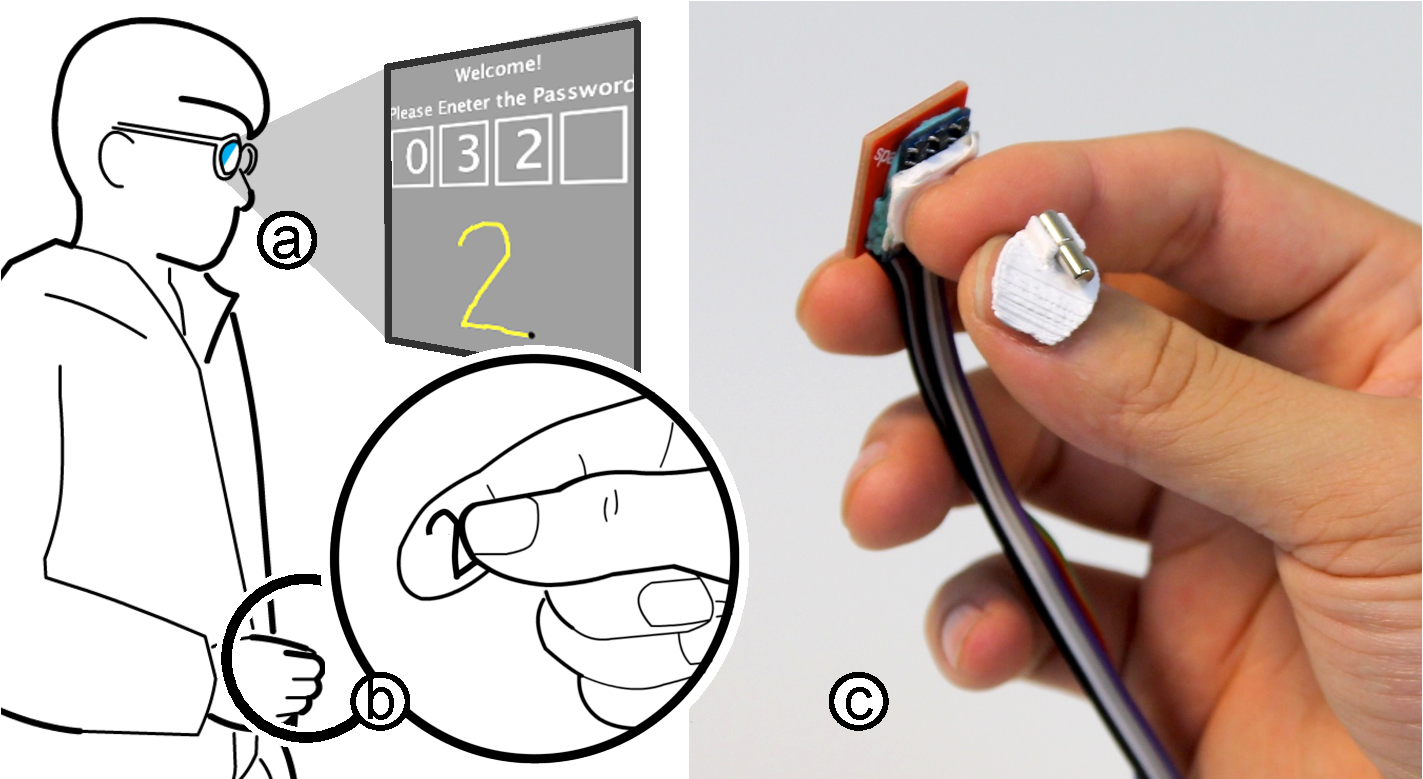
\includegraphics[width=1\linewidth]{firstFigure7}\\
   \end{tabular}
\caption{FingerPad enables touchpad function through the pinched fingertips using magnetic tracking, by adding a magnet and hall sensors on the fingernails, allowing for private and rich subtle interactions. Here, the user enters passwords to the (a) private glass display by (b) drawing numbers with the thumb tip on the index fingertip.}
\label{fig:firstFigure}
\end{center}
\end{figure}

%Human fingers allow for precise grasp of highest dexterity. This ability is a key to fine control of small tangibles. For instance, a small tangible pinched between thumb and fingers allows for arbitrary control of three-dimensional orientation.
%for grasping operations human hand has a high number of degrees of freedom, and there are many grasping styles depending on the shape of an object and purpose. 

Recent development in mobile computing proposes glass-mounted displays. 
Though similar to head-mounted displays, glass-mounted displays (e.g., Google Glass) are specially designed to be light-weighted, attachable, nonobstructive to natural vision, and with increased social acceptance. 

Although displays of this kind allow for personal and private visual outputs, their input methods may not keep the same level of privacy.
Voice input, for example, is commonly used for glass-mounted displays because it is expressive and effective. However, voice input can be problematic in loud environment, and inappropriate in public space when privacy is required (e.g., password input) \cite{Sawhney:2000}. 
Gesture input receives the similar privacy concern, because the input behaviors are easily observable.

%Subtle interactions rely on implicit movement as input, and are generally considered social acceptable. 

To allow for private input, recent research proposes subtle interactions \cite{Costanza:2007}\cite{Saponas:2009}\cite{wolf2011microinteractions}, which looks upon implicit movements and are generally considered socially acceptable. 
For example, muscle interface \cite{Saponas:2009} allows to input through unobservable muscle movement.
Foot gesture \cite{Scott:2010} detects subtle foot motions.
Ring devices \cite{Ogata:2012, Ashbrook:2011} and fabrics \cite{Karrer:2010} are developed to support tapping, spin, and slider inputs. %subtle and socially acceptable.
Although these methods allow subtle inputs (thus, private and socially acceptable), they generally suffered from limited input space.

%Input through implicit foot gestures \cite{Scott:2010} are not easily observable. 
%Input through finger rings \cite{Ogata:2012, Ashbrook:2011} or pinch fabrics \cite{Karrer:2010} are subtle and also socially acceptable.


% and are generally considered socially acceptable
%Foot gestures \cite{Scott:2010} are not easily observable. 
%Ring devices are developed to support tapping and spin input \cite{Ogata:2012, Ashbrook:2011}.
%Pinched fabrics \cite{Karrer:2010} allows for 1D slider input.


%Pinstripe \cite{Karrer:2010} allows 1D slider through pinched fabrics.
%or by implicitly move some body parts \cite{Scott:2010}.


%To allow for private input, researchers proposes subtle interactions \cite{Saponas:2009}\cite{wolf2011microinteractions}.


%In addition to privacy, social acceptance is another concern for the input methods. 
%Recent research proposes subtle interactions \cite{Saponas:2009}\cite{wolf2011microinteractions}.

%input through fabrics

%, not easily extensible for rich interactions. 



%previous subtle interactions only allows for limited input space, not easily extensible for rich interactions. 

%Subtle interactions \ref{Saponas:2009} are proposed as the mean to mitigate this concern.




% readily available
%There are situations where users were intended to access user controls at given posture. For instance, lying in bed, the user waken by an alarm strugglingly searches for the phone to set-off. This requires the effort to retrieve the devices (e.g., the phone). Always-available input \ref{Saponas:2009}[N] mitigates this effort by moving user controls to wearable devices which are easily accessible. 

%By removing this effort, users can save time and reduce errors (where is the error?).

% pinch gesture is natural.  ready for input.

% finger-worn device maximize availability / accessibility

%Instrumenting devices around fingers maximize the accessibility.

%even useable in no-hand situation

%Finger-worn device

%availability

%Always-available input \ref{Saponas:2009}[N] mitigates this effort by moving user controls to wearable devices which are easily accessible. 

% minimal travel distance, but not allowing rich interaction 
%Nevertheless, not all wearable devices are readily available. This availability depends on the effort to reach to the device controls. 
%To reduce this distance, previous works implement input functions around the users' hands. (Armtech) MuscleInput \ref{Saponas:2009}, for example, allows the wrist bend devices to read muscles movement as input. (FingerTech) Finger ring devices are developed to support tapping [iRing], 1D rolling \ref{Ashbrook:2011}, and marking menus through the ring.  These methods allow to input with little efforts, but provide limited input space, not easily extensible for rich interactions. 

%Wrist-watch touch screens, for example, require users hands traveling to the touchscreen, which introduces efforts. Gesture inputs \ref{Rekimoto:2001}\ref{Kim:2012} effectively increase availability with zero travel distance, but requires users to memorize functional mappings. 


%To support complex inputs, touch-based watch-display seems  a feasible solution, nevertheless, requiring the effort to reach to the touch screen.

%here, highlight strength of FingerPad.
%reach to FingerPad is a pinch-away. 


%\subsubsection{FingerPad}



%Benefits of FingerPad
We present FingerPad, a nail-mounted device that turns pinched fingertips into a touchpad, allowing for private and rich subtle interactions. As illustrated in Figure \ref{fig:firstFigure}, the user treats the index fingertip as the touchpad, and the thumb as the touch stylus.
FingerPad enables the touchpad function using magnetic tracking, by adding a magnet and hall sensors on the fingernails. 
Functionally, FingerPad is equivalent to a touchpad that users can learn with minimal effort.  Allowing for 2D touch inputs, FingerPad is ready for rich interactions including pointing, marking menu, and stroke input. 

%Unlike touchpads where fingers are styluses, FingerPad could interpret a finger pinch as the thumb touching the index fingertip (e.g., thumb as stylus, and index fingertip as touchpad), and vice versa. In this work, we identify two primary uses of FingerPad, namely IndexPad and ThumbPad. The two models both exist, and only in users� heads. Wrong model applied in FingerPad leads to inverted interpretation of touch positions. In the explorative study, we found the model applied in users� heads is related to the context of use, and highly affected by their experience in using touchpads. One primary factor is the orientation of fingers in use of FingerPad. For example,  touchpads typically faces up that fingers can effortlessly touch down. We will discuss more details in the study section.

%The rest of the paper is arranged as follows. First, related work is discussed. Then, the design of FingerPad is introduced and several example applications are presented to illus trate the enabled design space. Then, the underlying mechanism is detailed, including an evaluation and an examination of limitations, and the feedback of users, gathered from the explorative study is presented. Finally, conclusions are drawn and directions of future work suggested. 

\subsubsection{Benefits and limitations}
Allowing for touchpad functions through the fingers in pinch suggests several benefits. (1) Private: the movements of the fingers in pinch are subtle and naturally occluded by the operation hand. (2) Rich: the touchpad function allows input techniques, such as pointing, marking menu and stroke input. (3) Eyes-free: users can perform pinch gestures without visual support. (4) Natural haptic feedback:  by attaching on the nails, we preserve the natural haptic feedbacks on the fingertips, not affecting native functions of fingertips (e.g., grip small objects).
Additionally, by tracking through magnetism, FingerPad is occlusion free (i.e., can use with hand in pocket).



\subsection{SCENARIO}
\begin{figure}
\begin{center}
  \begin{tabular}{@{\hspace{0.1cm}}c}
		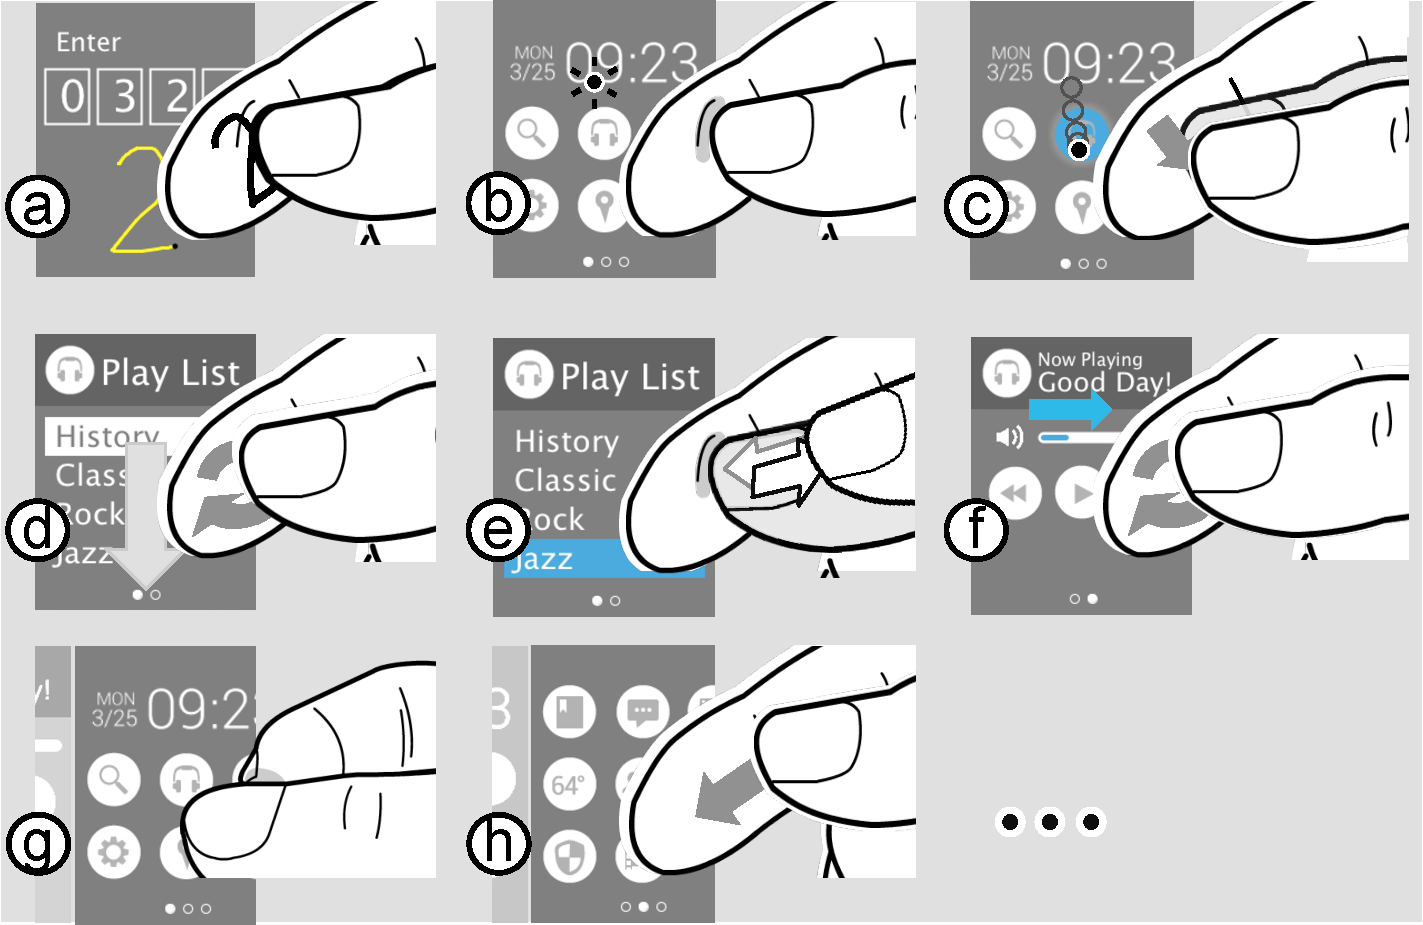
\includegraphics[width=1\linewidth]{walkthrough4}\\
   \end{tabular}
\caption{The walkthrough illustrates the use of FingerPad for glass displays. The graphics on the left-hand side of the subfigures are GUIs presented in the glass display view. The graphics on the right-hand side of the subfigures are the suggested gestures that can be enabled through our technique. }
\label{fig:walkthrough}
\end{center}
\end{figure}

Figure \ref{fig:walkthrough} illustrates a scenario of FingerPad for private visual outputs, such as the glass-mounted displays.
On the train on his way to work, Robin puts on the glass display. 
On the screen, the glass asks Robin the password for authentication. Instead of using voice input, he chooses to use the FingerPad input for privacy concern. 
(a) He writes four numbers, one by one, on his index fingertip, to unlock the glass application. 
(b) Robin long presses on the index fingertip to enter the cursor mode, (c) moves the cursor over the music app, and takes off the thumb for selection.
(d) In the music list, he circles on the fingertip to move to jazz category, and (e) clicks to enter the player page. (f) He circles again to tune up the volume. (g) To jump to home screen, he taps on the tip of the index finger. Now, he swipes the thumb leftward, moving to next app pages and plans to check the schedule of the day.

%(a) The user wrote password words on the fingertip to unlock the glass display, (b) long pressed to enter the cursor mode, (c) moved over music app, and taken-off for selection. (d) Circling on the fingertip, the user pulled down the list until Jazz, (e) single clicked to enter the player page. (f) After playing the music, he tuned up the volume by circling. (g) Tapping on the very end of the fingertip bring the display to home screen. (h) He slid leftward to second page, and started to check schedules of the day.
%\section{PILOT STUDY}
%Owing to natural bio-mechanism of human hands, using the index fingertips as  touchpads confronts unique usability concerns. %is not as easy as conventional touch pads.
%Firstly, unlike flat touch pads, fingertips are soft and curve, causing regions in the index fingertip not equally reachable by the thumb. Secondly, unlike touchpads, the motor space in the index and the thumb fingertips (i.e., the pad and the stylus) are constrained because they are mechanically connected by joints. 

%inter-connected, due to motor space of the two fingers is constrained due to the fact that the index and thumb are mechanically connected by joints. %Both make the touch regions in index fingertips not equally attainable.
%visible by the user eyesights and 

%To understand how to design touch interface for finger pads, we conducted a pilot study to determine the comfort levels in fingertip regions, as shown in Figure \ref{fig:pilotStudy}. 

%The participant was instructed to tap on regions in the index fingertip using the thumb tip. 
%To control the touch positions across participants, we stick thin translucent dot pattens  of their size (Figure \ref{fig:pilotStudy}a) on their index fingertips. 

%We divided the index fingertip into a 4 by 4 grid; each cell was represented by a dot. In task 1, the participants pressed the dots (three repetitions each cell, randomized) indicated on the screen. In task 2, they wrote a series of numbers on the fingertip. Participants performed the task without looking at their input fingers.

%The 4 by 4 dots evenly arranged across the fingertip. 
%, wrote a series of numbers on the fingertip (Figure \ref{fig:pilotStudy}c), and ranked comfort levels in the regions suggested by dots. %guide the participants the touch positions

%There were two tasks. In the first task, the participants pressed the dots indicated on the screen (Figure \ref{fig:pilotStudy}b), and wrote a series of numbers on the fingertip (Figure \ref{fig:pilotStudy}c). In the second task, we played an animation in which a cursor moved over a button and committed the selection. The participants emulate the effect  by performance using the pinched fingertips. A questionnaire followed up the study.

%\begin{figure}
%\begin{center}
%  \begin{tabular}{@{\hspace{0.1cm}}c}
%		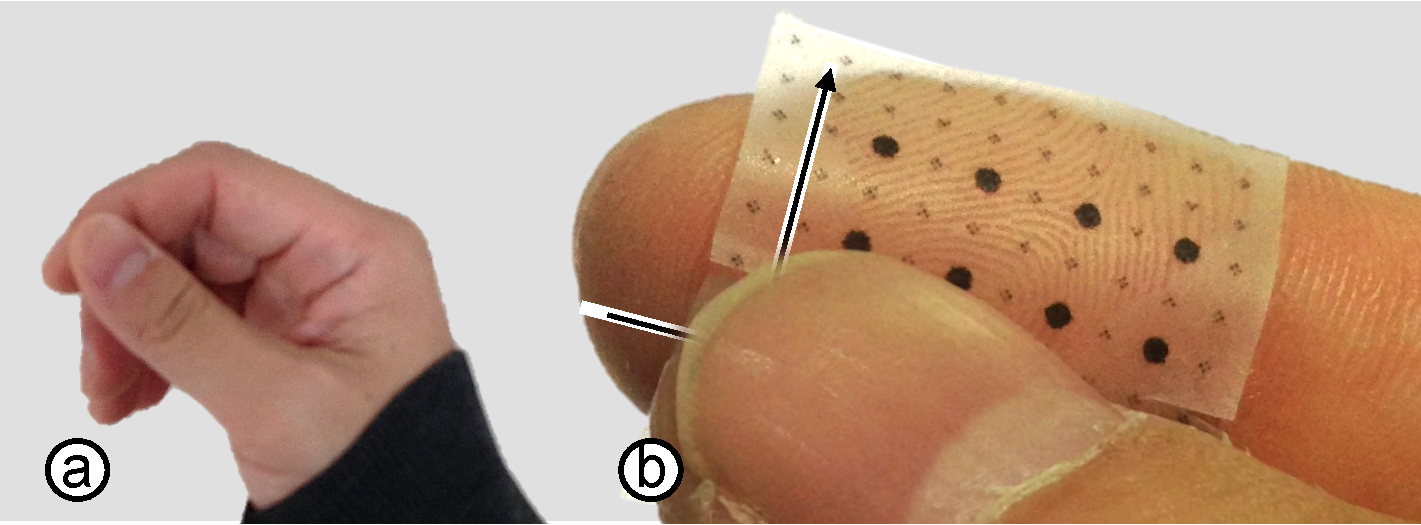
\includegraphics[width=1\linewidth]{pilotStudy}
%   \end{tabular}
%\caption{(a) The posture the participants were instructed to perform in the pilot study. (b) The translucent dot pattern stick on the fingertip to guide the participants through touch.}
%\label{fig:pilotStudy}
%\end{center}
%\end{figure}

%\begin{figure}
%\begin{center}
%  \begin{tabular}{@{\hspace{0.1cm}}c}
%		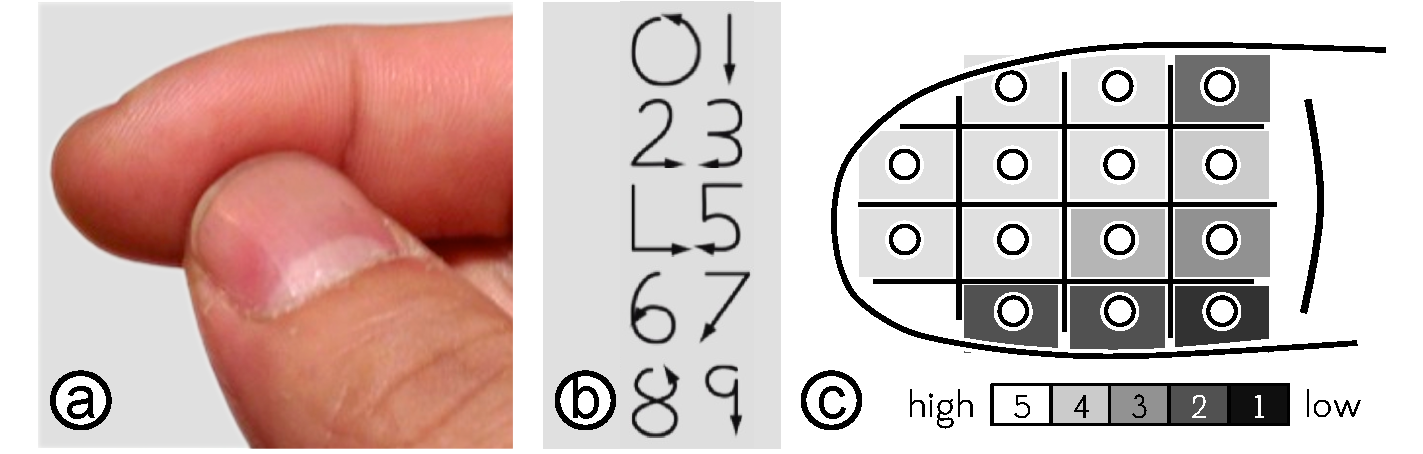
\includegraphics[width=1\linewidth]{pilotStudy5}
%   \end{tabular}
%\caption{(a) The pilot study includes two tasks: (a) the tapping task and (b) the drawing task. (c) Participants rank comfort levels of touch in the regions across the index fingertip.}
%\label{fig:pilotStudy}
%\end{center}
%\end{figure}

%\subsection{Result \& discussion}
%7 participants (3 females), between 22 and 34, were recruited, all right-handed. 2 female participants had long nails.
%Figure \ref{fig:pilotStudy}c shows the average comfort levels across regions in the index fingertip. Brighter region indicates higher comfort level.
%The result reported that the inner regions (lower-right regions) in the index fingertips in general received lower comfort levels than the outer regions. 
%The participants who had this tendency described that it required additional force to bend thumb limbs in order to reach the dots at the bottom row and, in particular, the dot at bottom-right corner.

%\subsubsection{Bent or hunched postures}
%We found two primary types of thumb-as-stylus postures that affected the comfort levels. 
%The participants either (a) bent the thumb (Figure \ref{fig:twoTypesOfThumb}a) such that the thumb tip pointed from below the index fingertip, or (b) hunched the thumb (Figure \ref{fig:twoTypesOfThumb}b), allowing to point from above.
%The participants (3 out of 7) who applied bent postures gave 2.3 times lower in comfort levels at regions in the bottom row than the participants who applied hunched postures. With further instructions, all but one participants, who used the bent postures at trials, reported they can use the hunched posture without problems. 

%We also asked how they determined the touch positions through haptics. 
%In the regions easier reachable (e.g., the outer regions), participants with short nails determined the touch through the contact area close to the edge of the thumb tip, similar to the projection model suggested by Christian Holz \cite{Holz:2011}. This strategy switched to using sharp haptics through the nail edge, when their thumbs had extended nails.
%Two female participants who had long nails touched the bottom row regions using the nail back (\ref{fig:fingerpadFunction}a), which, to a large extent, degraded their sense of touch positions.

%\subsection{Touch Interface Design}
%As illustrated by Figure \ref{fig:fingerpadFunction}b, we divide the index fingertip into two functional regions: the pad and the bezel regions. The pad region covers the central and upper parts of the fingertip, suggesting a near flat and easily reachable area.
%In the bezel region, we install a big button on the bottom, and a button on the very end of index fingertip. The bezel buttons allow short cut operations, such as the \textit{home button} illustrated by Figure \ref{fig:walkthrough}g in the \textit{SCENARIO}.

%In \ref{fig:twoTypesOfThumb}a, the participants bent the thumb downward such that the thumb tip pointed from below the index fingertip. In \ref{fig:twoTypesOfThumb}b, the participants hunched up the thumb such that the thumb tip pointed from above. 

%\subsubsection{Friction}

%\subsubsection{Area of comfort}

%\begin{figure}
%\begin{center}
%  \begin{tabular}{@{\hspace{0.1cm}}c}
%		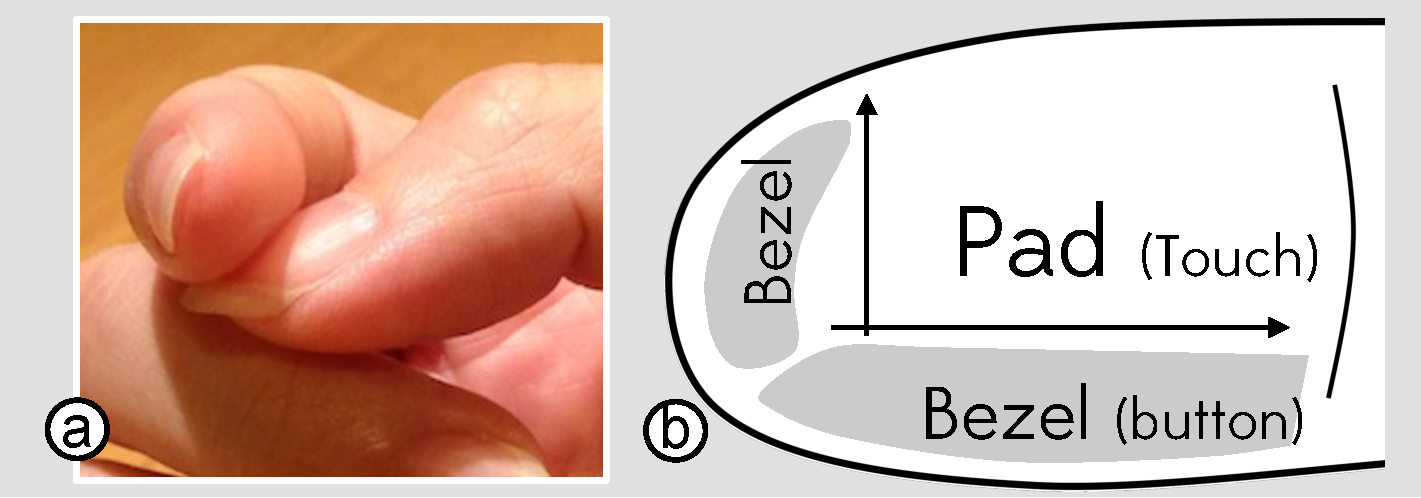
\includegraphics[width=1\linewidth]{fingerpadFunction8}\\
%   \end{tabular}
%\caption{(a) The participant with long nail touched the bottom regions with the nail back. (b) According to the pilot study, we divide the index fingertip into two functional regions: the pad and the bezel regions, for touch pad input and button input. }
%\label{fig:fingerpadFunction}
%\end{center}
%\end{figure}




%\subsubsection{commitment method}

%\subsubsection{Activation}



%\begin{figure}
%\begin{center}
%  \begin{tabular}{@{\hspace{0.1cm}}c}
%		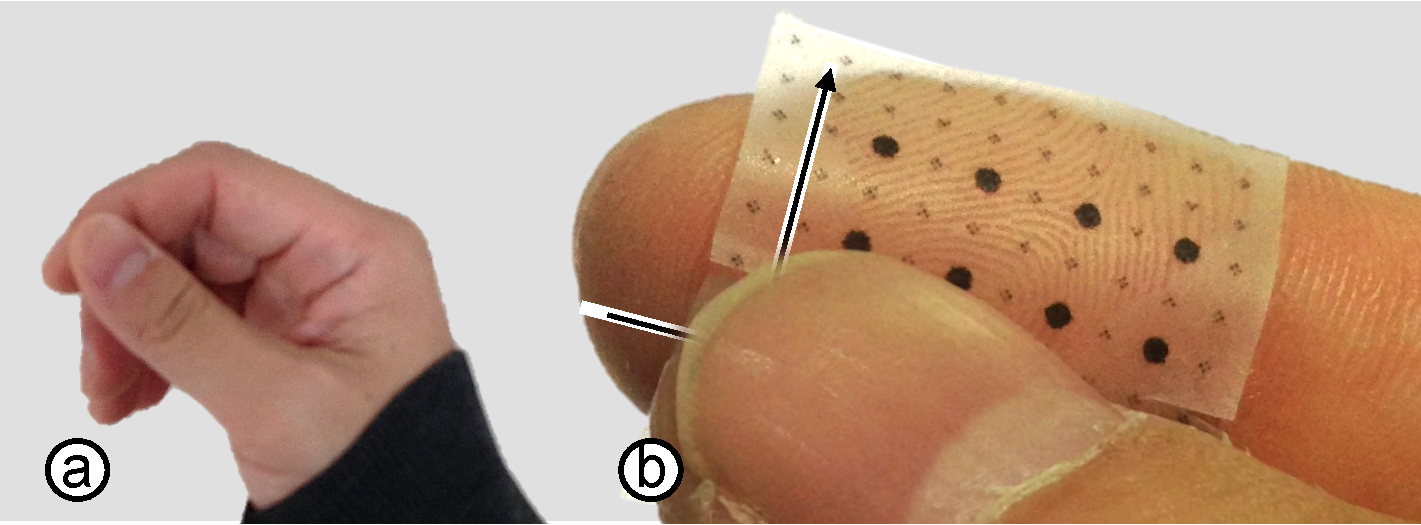
\includegraphics[width=1\linewidth]{pilotStudy}\\
%   \end{tabular}
%\caption{(a) The posture the participants were instructed to perform in the pilot study. (b) The translucent dot pattern stick on the fingertip to guide the participants through touch.}
%\label{fig:pilotStudy}
%\end{center}
%\end{figure}


%\section{DESIGN: IndexPad v.s. ThumbPad}
%Unlike touchpads where the finger is always considered as an input pen, FingerPad's  pad and pen, referring to index and thumb fingertips, are interchangeable. We include two models into consideration: IndexPad and ThumbPad, depending on which fingertip users perceive as the finger touchpad. Misinterpretation of the model applied can lead to inverted results. For example, on a finger pinch, the sense of touch is contributed from the contact regions locating at different parts in the index and thumb fingertips. These regions suggest different touch positions in both fingertips, as well as in the user's mental. Unfortunately, the model applied only exists in users head. Without understanding what might trigger the decision of the model to use, interaction with FingerPad can be frustrating. 

%To understand how users determine which model to use, and what pros and cons each model inherits, we conduct a pilot study.

%We argue that  this decision is affected by the orientations of the fingertips. Unlike touchpads which always face up allowing for touch, the orientation of FingerPad can be various depending on the context of use. The fact that wearing input devices on fingertips suggests using the device instantly at anytime, as shown in Figure \ref{fingerPadPosture}, making this worse.

%Moreover, unlike touchpads which always face up allowing for touch, the orientation of FingerPad can be various depending on the context of use. 
%Depending on the context of use, FingerPad's orientation can be various yet unexpected. 
%The key seems to understand  when and why users perceived their fingertips as the pads.
%Moreover, the fact that wearing input devices on fingertips suggest using it instantly at anytime makes this worse.
%FingerPad allows two distinct interpretations of touch. 

%\label{fig:typeOfPads}

%\subsection{Functional regions}
%Center and upper area receive good comfort level in touch. Lower part is not easily seen. Very lower part often tapping with nail back. Left part taping with thumb tip side. Show several examples in Figure \ref{fig:functionRegion}a.

%As suggesting by the results, we divide the index fingertip into two functional regions: the touch pad , and the bezel buttons, as shown in Figure \ref{fig:functionRegion}b. The pad region suggests a flat surface that maximize visibility and facilitate touch behavior. The bezel regions, on the tip and lower part of the index fingertip, allows buttons to e.g., invoke menus. While the lower part seems wide enough to embed more buttons, we simplify it to single big button because the comfort level is low and the way users might touch it is versatile.

%\begin{figure}
%\begin{center}
%  \begin{tabular}{@{\hspace{0.1cm}}c}
%		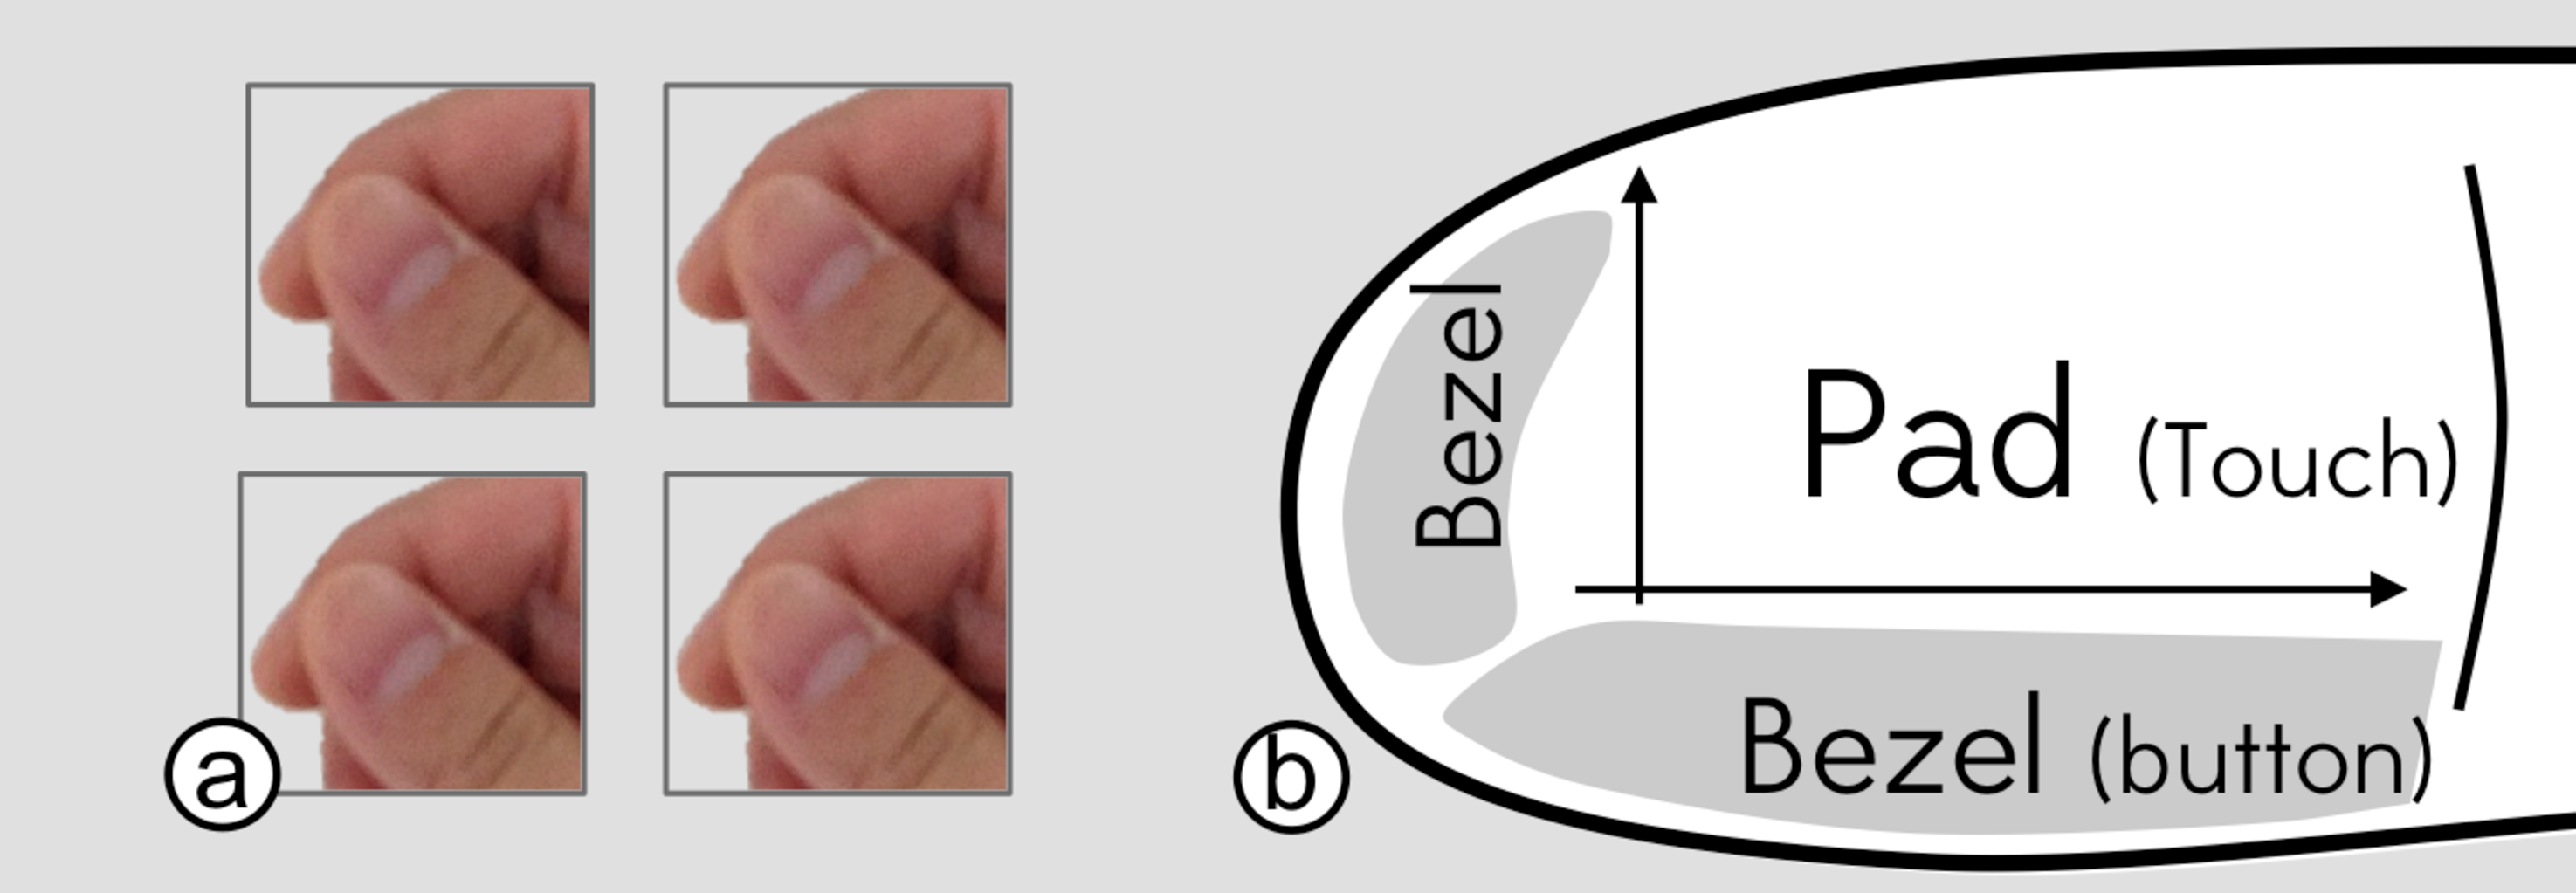
\includegraphics[width=1\linewidth]{fingerpadFunction7}\\
%   \end{tabular}
%\caption{(a) Example postures of the thumb tapping at tip and lower part of the index fingertip. (b)Design of functional regions in FingerPad.}
%\label{fig:functionRegion}
%\end{center}
%\end{figure}


\section{PROTOTYPE}
%; it turns index fingertip into a touchpad, by attaching the sensing plate on the user' index fingernail and the magnet on the thumbnail (Figure \ref{fig:firstFigure}). 
FingerPad is a pair of nail-mounted devices comprising of a thin (1mm) magnetic sensing plate, and a plate of ferromagnet. 
The sensing plate includes a 3x3 Winson WSH138 Hall sensor grid (Figure \ref{fig:hallDevice}a), and each sensor is separated to each other by 2mm, which suggests an area of 12(W) mm x 12(H) mm. 
Each sensor element detects both N- and S-polar magnetic field intensities in a range from 0 to 200 Gauss on a 1024-point scale. 
An Arduino board with an ATmega32U4 microprocessor is used to bridge the sensing plate with the computer.
According to the magnetic strength captured by the plate, FingerPad approximates the magnet's position, transforms the position to the finger-pad coordinate defined through user calibration (see  \emph{Tracking} and  \emph{User calibration}), and sends to the applications. 

\begin{figure}
\begin{center}
  \begin{tabular}{@{\hspace{0.1cm}}c}
		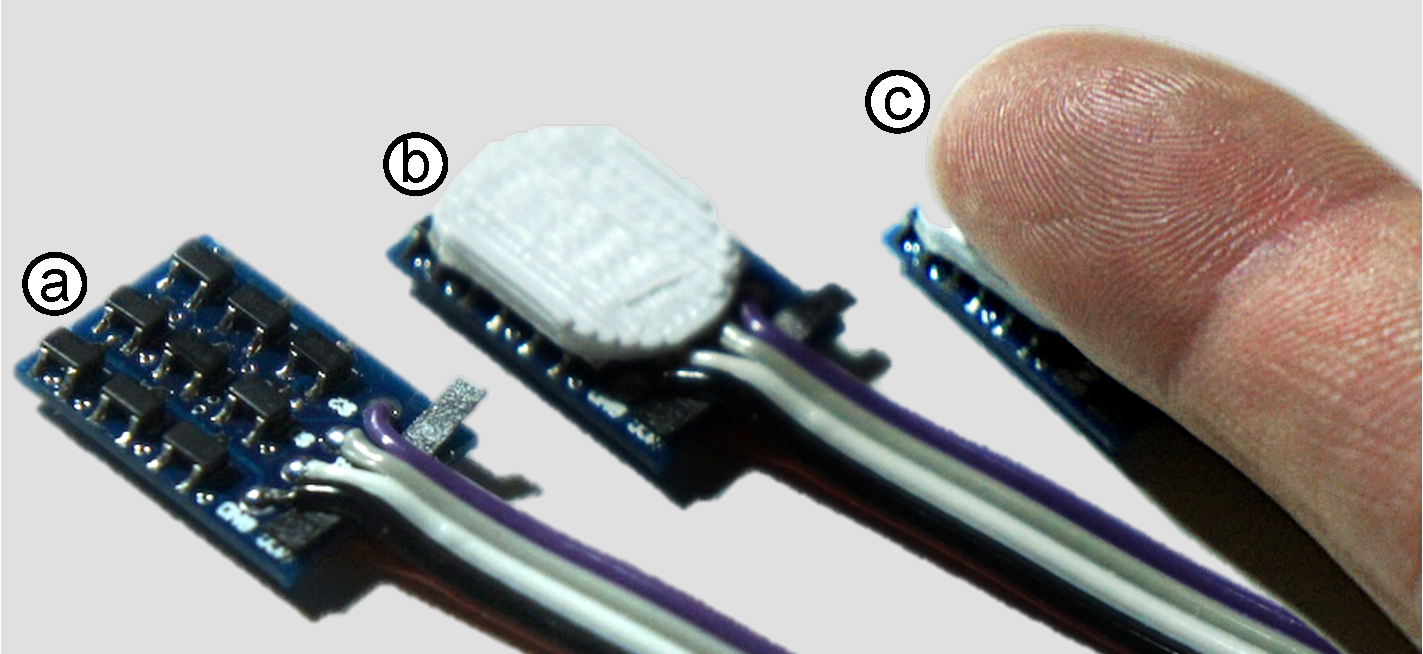
\includegraphics[width=1\linewidth]{hallDevice}
   \end{tabular}
\caption{(a) The 3x3 hall sensor grid, and (b) a nail-shape plate with a curve surface (c) suggesting fitness to the natural nail. }
\label{fig:hallDevice}
\end{center}
\end{figure}

\begin{figure}
\begin{center}
  \begin{tabular}{@{\hspace{0.1cm}}c}
		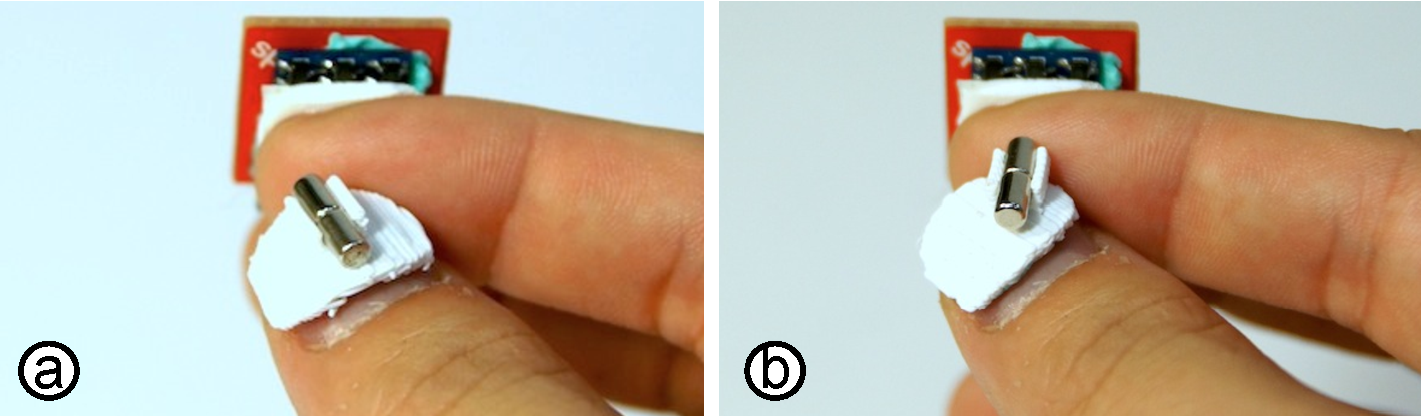
\includegraphics[width=1\linewidth]{magnetHolder3}
   \end{tabular}
\caption{The magnet holder grips the magnet at certain orientation. 
(a) The first design of the magnet holder. (b) we push the magnet orientation 30 degree to the right, accommodating to the bio-mechanism of the index and thumb fingers.}
\label{fig:magnetHolder}
\end{center}
\end{figure}

To attach the sensor plate firmly on the nail, we use a 3D printer to craft a nail piece that suggests a nail-fit curve surface. 
As shown in Figure \ref{fig:hallDevice}b, the sensor plate, gluing with the nail piece, is further glued on the user's nail using a twin adhesive tape. 
By gluing, we help users envision the future nail devices akin to the use of the artificial nails.
We put on the prototype on the user's index fingernail in a way that the wires would not affect the finger motor space.

We create another nail piece that holds the magnet and fixates the magnet orientation. 
The principle to place the magnet is to allow the polar orientation of the magnet in parallel with the normal of the sensor grid when users placing the thumb on the center of the index fingertip. 
Figure \ref{fig:magnetHolder}a shows our first design. 
To adapt the bio-mechanism of the thumb and index finger, we improve the design by moving the magnet orientation 30 degree to the right (Figure \ref{fig:magnetHolder}b). 
%This way, we improve and maximize the tracking range.

The magnet we used is a 2mm disk x 8mm strong ferromagnet, which allows for effectively sensing within 2.1cm by our sensor plate.
% allowing for the magnetic field remotely visible to the hall sensor plate on the index fingernail.
Note that this effective distance can be further extended by using more sensitive magnetism sensors, such as magnetometers \cite{Ashbrook:2011}.
% and maximizing the user envisioning the future device.

%This instrument is not suitable for measuring weak fields, such as the geomagnetic field.

%\subsection{Future device}
%show photo of skin-thin hall sensor grid. 



\subsection{Tracking}
We define a cartesian coordinate for the sensor-grid coordinate. 
For the 3 by 3 sensor grid, the sensor at the lower left corner is set as the coordinate origin. 
We approximate the magnet position in the sensor-grid coordinate using bilinear weighting according to the magnetic strength read by each hall sensor. 
Because the read magnetic field strength is in fact a mix of quadratic and cubic attenuation, this approach can only approximate the magnet position. 
We further regulate the positioning result in the \emph{User Calibration} section.

To improve the positioning, two strategies are applied. 
First, the polar of the magnet is placed in parallel with the normal of the sensor grid as shown in Figure \ref{fig:magnetHolder}b.
Second, we exclude the opposite polar values read by the sensors. 
When users tap on the edges of the index fingertip (e.g., the tip or bottom areas), 
the magnet orientation may deviate from the normals of the sensors, which causes some sensors read the opposite polar values. %and confusing the positioning.

%Third, we restraint the sensing area to only around the 

% As a result, we can reliably compute the magnet position in the sensor-grid coordinate.

\subsection{User calibration}
The purpose of user calibration is to regulate the 2D positions computed in \emph{Tracking}, to the finger-pad coordinate in the index fingertip.
%, to (2) maximize the use of real estate in the user's fingertip.
To account for the non-linear mappings between the sensor-grid and the finger-pad coordinates, we divide the finger-pad coordinate into multiple sub-coordinates, and approximate the nonlinearity by computing homographic transformation between each sub-coordinate and the sensor-grid coordinate. 
%This piece-wise approximation allows us to reduce the transformation errors.

\begin{figure}
\begin{center}
  \begin{tabular}{@{\hspace{0.1cm}}c}
		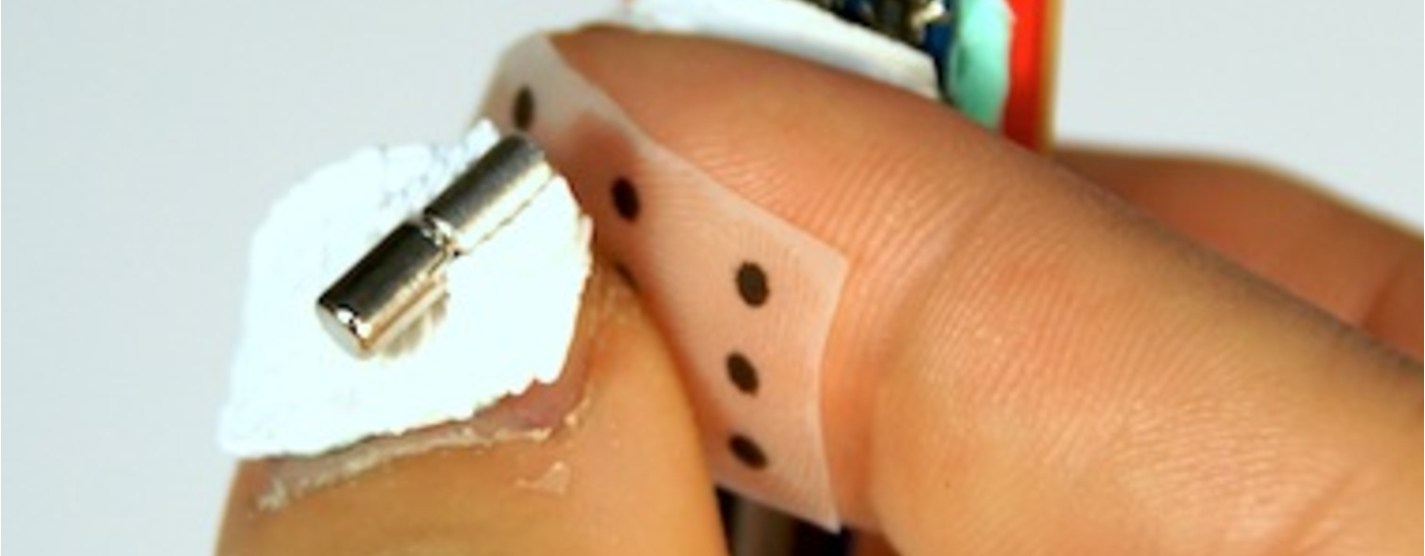
\includegraphics[width=1\linewidth]{userCalib3}\\
   \end{tabular}
\caption{To guide the calibration process, we stick a translucent dot pattern on the index fingertip, that helps to obtain good homographic transformations.}
%\caption{The participant's fingertip is sticked with a translucent pattern for touch positioning. (a) Translucent dot patterns in different fingertip sizes. (b) Edges of the pattern is cut open in order to fit curve surface of fingertip.}
\label{fig:userCalib}
\end{center}
\end{figure}

Typically, a homographic transformation can be determined by more than 4 pairwise correspondent points. 
To guide the calibration process, we stick a translucent dot pattern on the index fingertip. 
The dots are separated by 4mm in a Cartesian coordinate, and the 3 by 3 dot pattern suggests a normal size of the fingertip. 
We stick the pattern on the index fingertip area, as shown in Figure \ref{fig:userCalib}. 
The 9 pairs of the correspondent points from calibration process are then used to compute the homographic transformation for each of the four sub-coordinates. 
As long as the magnet orientation correctly positioned, the calibration configuration can adapt well to fingers with different sizes and thickness.
% only if the magnetic field is still sufficiently visible.

%Because the nail is typically smaller than the finger pad, when tapping to the edges of the index finger pad, the magnet may point outside of the proper range of the sensor grid, and affect the positioning result.

%We use the same translucent stick but in different dot pattern, to guide the user through calibration.
%The dots, separating by 2mm, form a cartesian coordinate (Figure \ref{fig:userCalib}a); a 3 by 4 dot pattern suggests a normal (need detail) finger size. (how to deal with different finger size?)
%To accommodate different finger sizes, we increase the pattern size by adding more dots, which increases user efforts in calibration but minimizes the positioning errors. 
%As in pilot study, we glue the pattern on the user's index fingertip in a way that keeps the bezel area clean (Figure \ref{fig:userCalib}b).
%During calibration, we instruct the user to press each dot and bezel button once with the thumb tip. Our system records the positions computed from \emph{Tracking} and the dot positions in the finger coordinate.


\subsection{Land-on detection}
Although the hall sensor plate can detect hover state (e.g., the thumb is in the proximity to the index fingertip) according to the strength of the magnetic field, it is hard to determine when the user's thumb landing-on the index fingertip.
To detect land-on, we add an accelerometer to the hall sensor plate to detect the impact of the finger contacts.
For the detail, we compute the derivative in the X, Y, and Z-axes, respectively, by using a sliding window. 
Through monitoring the values in the sliding window, a candidate for land-on can be found when a positive derivate is followed by a negative derivative.
A land-on action is only reported, when the thumb is found within the hover range at the same time.
After land-on, touch interactions performed by the user can be recognized, until the thumb is out of the hover range.

\subsection{Flick selection}
We propose the flick selection, as shown in Figure \ref{fig:flickSelection}.
Moving the cursor over a target, the user commits a selection by taking off the thumb up.
Upon exit of the hover state, we remove the cursor movement in the last 180 milliseconds (determined from a pilot testing) to eliminate the unwanted cursor movement. The last cursor position is used to determine the selection. 
The side effect of the flick selection is that the user may see the unwanted cursor movement before the thumb exits the hover state.
Nevertheless, the users can understand it and it won't affect users' performance.  

%Even though they understood these extra traces would not be counted in the selection process, the participants reported in our user study that they felt uncomfortable for this effect.

%\subsection{Choice of magnets}
%show a series of magnets, their 3d magnetic field shape, and the heights suggested.
%Rationalize why we choose the magnet in the prototype.


%While the Tracking reports 2d positions which are relative yet irregular (e.g., non-uniform), we regulate these positions by including manual calibration.

%To guide the user through calibration, we print a dot grid pattern on a translucent adhesive film. 


%\subsection{Evaluation}
%report errors with fewer calibration dots. using 2mm dot as ground truth.

\section{APPLICATION}
%To demonstrate FingerPad as an input method for the glass display, we implenment a glass interface using the LCD screen, as shown in Figure \ref{fig:glassUI}. 
Based on the touchpad functions provided by our prototype, we implement the touch cursor, gesture input, and stroke input functions to prove the capability of the FingerPad. 
The implemented application is the same as described in the \emph{SCENARIO} section.
 In the touch cursor function, a user can perform a long press to enter the cursor mode which reveals the cursor on the display (e.g., glass interface). 
 By moving the thumb on the index fingertip, the user can freely move the cursor. 
 Through the flick selection, the user can commit a selection on the menu. 
 For the gesture input, we also provide swipe and circling gestures. 
 In a page view, the user can swipe to left or right to enter the next or previous page. 
 In a list view, the user can perform clockwise or counter-clockwise circling gesture to scroll down or up through the list. 
 In stroke input, we adapt the unistroke recognizer \cite{Wobbrock:2007} for our numeric input, which allows users to write the password or phone numbers. 

\begin{figure}
\begin{center}
  \begin{tabular}{@{\hspace{0.1cm}}c}
		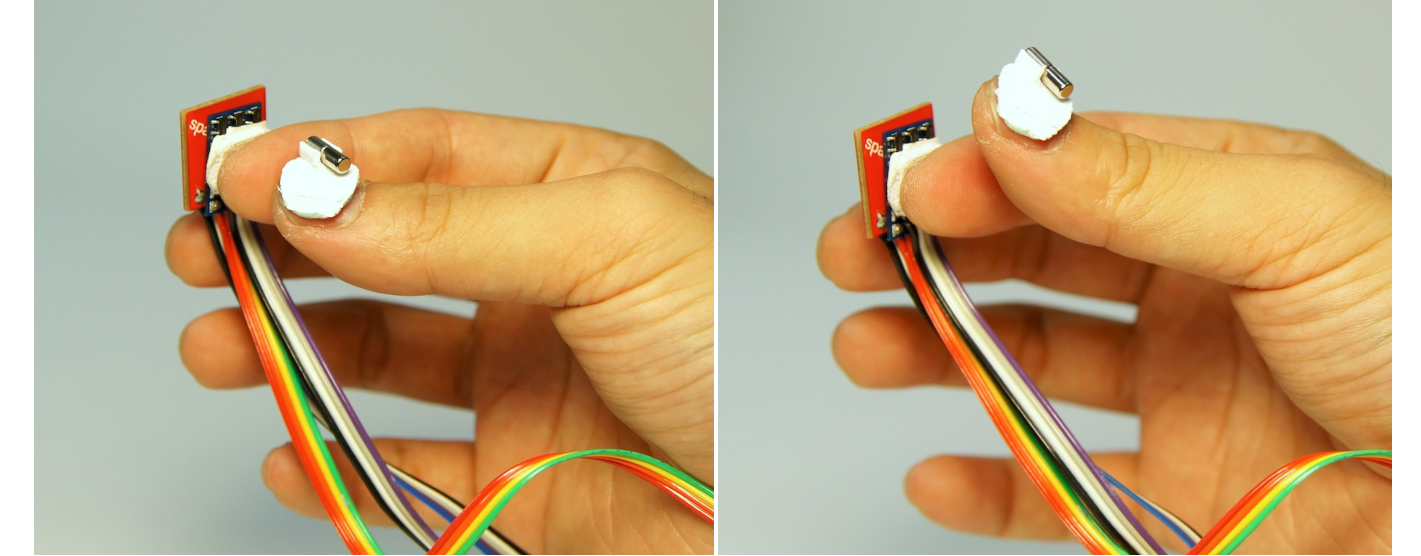
\includegraphics[width=1\linewidth]{flickSelection2}\\
   \end{tabular}
\caption{The user commits a selection by flicking the thumb up.}
\label{fig:flickSelection}
\end{center}
\end{figure}



%\section{USER STUDY}
%There are two studies.
%The purpose of the study is to determine users� ability to provide 2D input using FingerPad. 


%Two usage conditioned were included: seated and walking.
%Our goal was to understand how precise the participants can perform cursor control on the move.


\subsection{USER STUDY}

The purpose of the study is to determine users' ability to provide precise cursor control through the fingertips in pinch. 
Because the subtle interactions are designed for mobile usage, therefore, the seated and walking conditions are considered. 
The walking condition allows us to see the level of influence while using the FingerPad technique on the move with glass displays.
Moreover, the committed methods may also affect users' performance. 
Therefore, we not only tested flick method, but also tested bi-manual clicker method. 
Finally, we also want to know how small the target that the users can point at to know the limitation.  

%We performed the task under two conditions: seated and walking conditions. 
%The seated condition allows us to see how well participants used our techniques after training. 

%The walking condition reveals the level of influence from walking waving.
%A questionnaire followed the study.

%native user ability in cursor control because the button-press minimizes  the errors from commitment methods. 
\subsection{Task and Conditions}

The participants need to move the cursor over the target shown in the screen and commit the selection by using single-handed flick selection method or the bimanual clicker method with the non-pointing hand depending on the conditions. 
The target's color will be changed when the cursor is entered into the target square. 
Upon successful selection, the target will disappear and next target will be showed up on the screen.
We measured task time and error rate for the target sizes of 10mm, 5mm, 2.5mm, 1.2mm and 0.6mm separately. 
The 0.6mm case is included to test the users' limitation.

In the \emph{seated condition}, the participants sat on the chair in front of the table where the screen was positioned toward the them. 
They were instructed to adjust the chair height such that they could rest their dominant hands on the table for support (Figure \ref{fig:walking}a). 
The participants ensured that they could see the smallest 0.6mm target clearly. Otherwise we moved the screen closer to the participants. 
In the \emph{walking condition}, they performed the tasks on the treadmill. 
The screen was placed on top of the treadmill control platform, as shown in Figure \ref{fig:walking}b.
The treadmill was set to normal walking speed (3.5 km/hour). % with a range of 0.5km according to the participants difference. 

\begin{figure}
\begin{center}
  \begin{tabular}{@{\hspace{0.1cm}}c}
		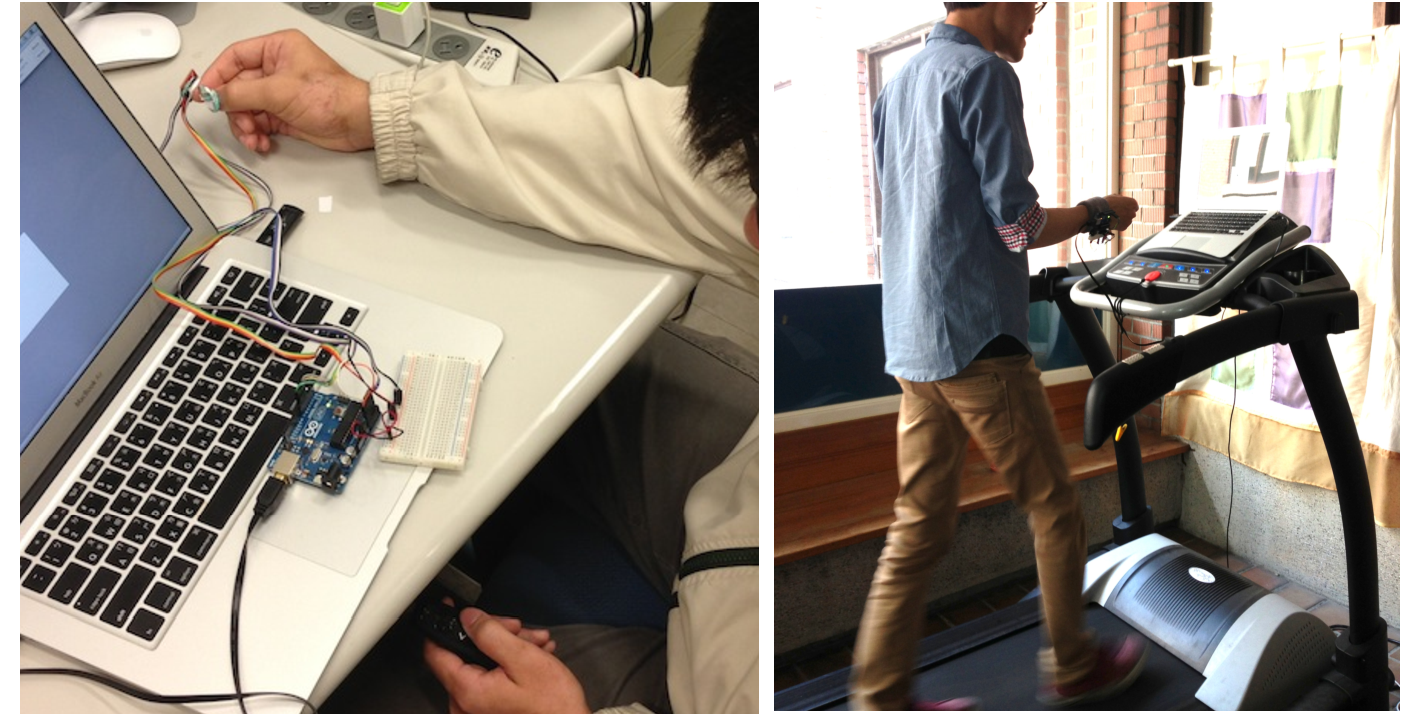
\includegraphics[width=1\linewidth]{walking3}\\
   \end{tabular}
\caption{The study setup for the seated (left) and walking conditions (right).}
\label{fig:walking}
\end{center}
\end{figure}

%\begin{figure}
%\begin{center}
%  \begin{tabular}{@{\hspace{0.1cm}}c}
%		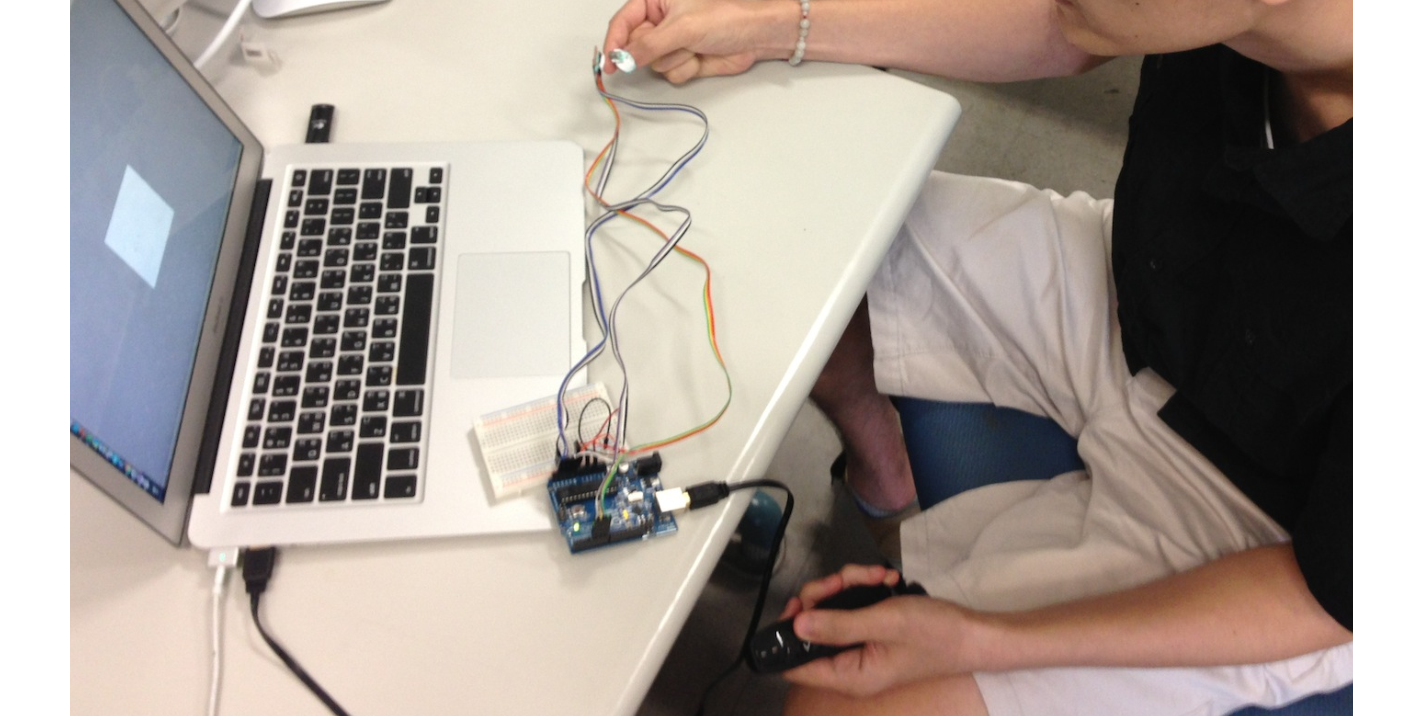
\includegraphics[width=1\linewidth]{seated3}\\
%   \end{tabular}
%\caption{The setup of our user study. (a) The screen, (b) the FingerPad device, and (c) the clicker in the non-dominant hand.}
%\label{fig:seated}
%\end{center}
%\end{figure}

\subsection{Interface and apparatus}

The participants wore the sensor part of the finger pad device on the index fingernail, and the magnet part on the thumbnail. 
Because the nail sizes and the way participants move their thumbs on the index finger pads are bio-mechanically different, we helped participants put on the device, and adjusted the magnet holder orientation in order to accommodate interpersonal tapping habits.
In the pilot testing, we found the thick fingers from some male participants could degrade the tracking performance with the original magnet setting. 
To avoid the tracking errors in the study, we replace the magnet with a wider magnet (4mm disk * 8mm height) that ensures the tracking performance in the study.
%In addition, we used a larger magnet (4mm disk * 8mm height) in the study. The stronger magnetic field makes sure participants with thicker fingertips work well, and improves cursoring stabilization.

\subsection{Experimental design}
%The experiment was a 5x2 within-subjects factorial design, with five button size conditions ( 11mm, 5.5mm, 2.8mm, 1.2mm, 0.6mm), and two commitment conditions (single-handed flick and bimanual click).
The study design was 2 x 2 x 5 x 12 (Condition x Commitment method x Target Size x Target Position) with 3 repetitions for each cell. The Condition was the between-subject variable. The target sizes were 10mm, 5mm, 2.5mm, 1.2mm and 0.6mm separately, and the  target positions were the 12 centroids of a regular 4 x 3 grid. 
For each trial, we recorded the task completion time and error. 
The different commit methods were counterbalanced. 
The target sizes and positions were randomized. %Participants received up-front training.

\subsection{Participants}
22 participants (10 female) with mean age of 26.9 (std: 3.9), between ages of 22 and 38, were recruited from the university. 
Each was rewarded a small gift for their participating. 
The task took about 30 minutes. 
All participants have the experience of touching input, because they all have touch-input smart phones.
All are right-handed.


\begin{figure}
\begin{center}
  \begin{tabular}{@{\hspace{0.1cm}}c}
		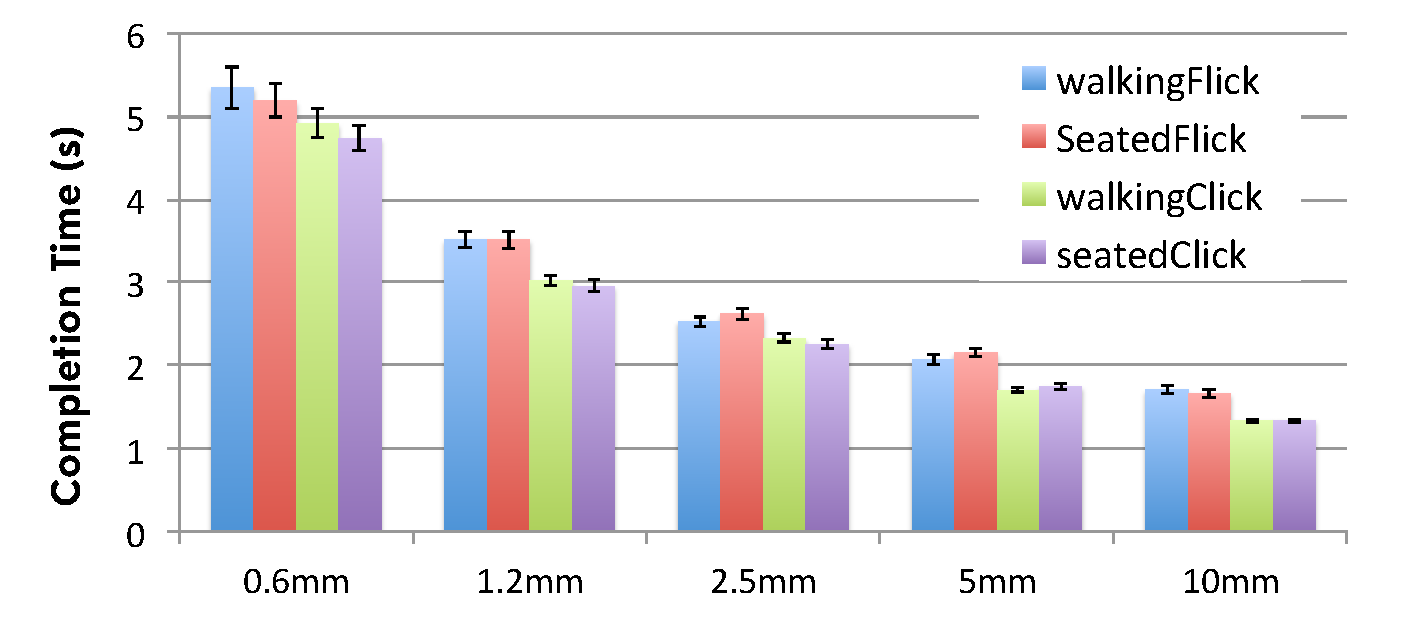
\includegraphics[width=1\linewidth]{completionTime}\\
   \end{tabular}
\caption{The study completion times, with 95\% confidence intervals, of different target sizes in two commitment methods under seated and walking conditions.}
\label{fig:completionTime}

\end{center}
\end{figure}
\begin{figure}
\begin{center}
  \begin{tabular}{@{\hspace{0.1cm}}c}
		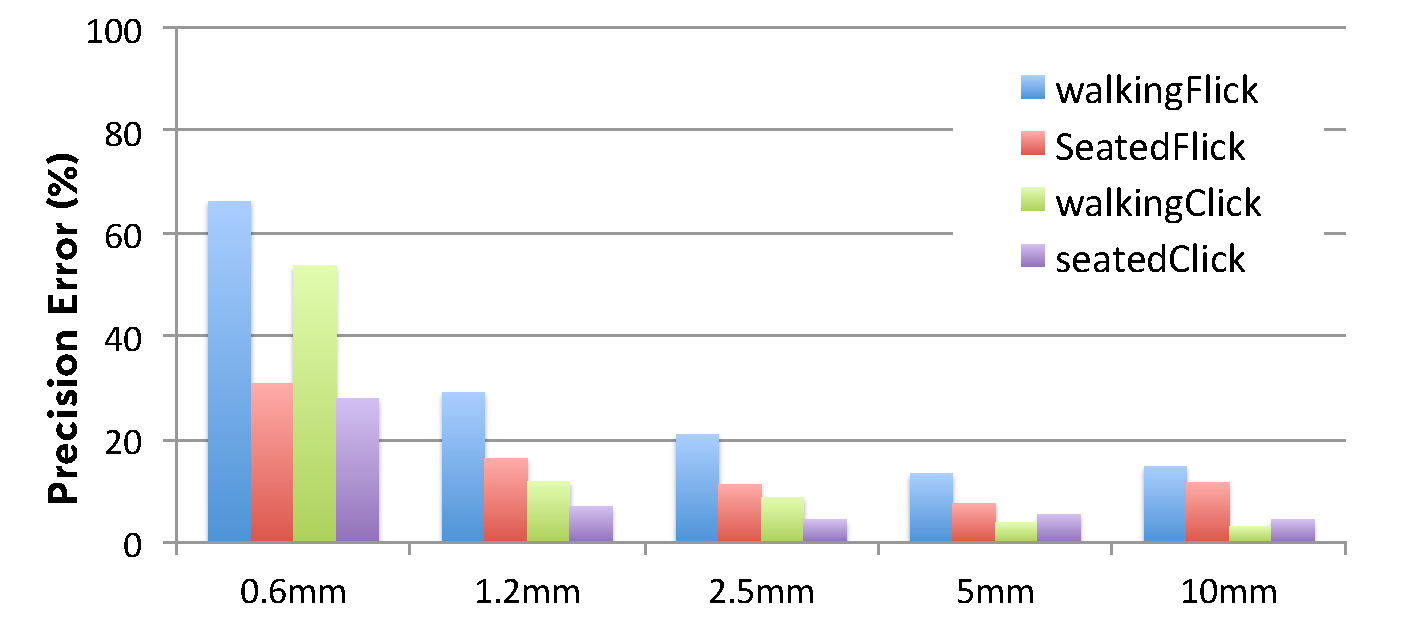
\includegraphics[width=1\linewidth]{errorRate}\\
   \end{tabular}
\caption{The study error rates of different target sizes in two commitment methods under seated and walking conditions.}
\label{fig:errorRate}
\end{center}
\end{figure}


\subsection{Results and discussion}
%For four different conditions (i.e. walkingFlick, walkingClick, seatedFlick, and seatedClick), the smaller the target size, the more time participants needed to take to complete the task (M = 1.5s for 10.0mm, 1.9s for 5.0mm, 2.4s for 2.5mm, 3.2s for 1.2mm, and 4.9s for 0.6mm across all conditions). 

%There were no significant difference between four conditions for target size 0.6mm, 1.2mm, 2.5mm. While for the target size of 5.0mm, the post host Bonferroni test showed that there were not significant between �seating� and �walking� conditions for both flick (M = 0.07s v.s. 0.13s, p = 0.30) and click (M = 0.05s v.s. 0.04s, p = 3.66) commitment approaches. 
%For the target size of 10.0mm, similar results had been discovered (M = 0.11s v.s. 0.14s, p = 0.10 for flick. M = 0.05s v.s. 0.03s, p = 3.81 for click).

%There were no significant differences (p < .05?) between the seated and walking conditions.
 

%%% Same size: Same interaction method: different posture: compare the complete time & error rate 

\subsubsection{With the same target size, the same commitment method, but different postures}

To analyze the obtained data, we ran the t-test pairwisely to know whether the different postures will affect the users' performance. 
The statistics shows that no matter the condition is walking or seated, the completion time has no significant difference. 
However, for error rate, when the target size is below 2.5mm, it shows the significant difference between the two different postures. 
For the design insight, if the system can detect users' postures, it can provide different UI layouts when users are in different postures. 
For example, while users are seated, the system can provide tight layout and compact information, and while users are walking, the system can provide loose layout and abstract information. 
However, if the users want  the consistent user experience, the target size should be above 2.5 mm.


%%% Same size: different interaction method: same posture: compare the complete time & error rate 

\subsubsection{With the same target size, the same posture, but different commitment methods}

To analyze the obtained data, we ran the t-test pairwisely to know whether the different commitment methods will affect the users' performance. 
For the completion time, the statistics shows that there is a significant difference only in the condition while the posture is walking and the target size is 10mm.
Therefore, we can say that generally the two different commitment postures don't affect the performance of the completion time. 
On the contrary, for the error rate, except the 0.6mm case, while in the walking condition, the statistics shows significant difference between flick and clicker methods. 
For the design insight, we can conclude that if we want to improve the performance, we can choose the different commitment methods. 
However, there is a trade-off between the two methods. 
Though the clicker method can achieve better performance, it requires bimanual interaction. 
Compared to clicker method, users can performance the task with only one hand, which provides more freedom to the other hand.

\subsubsection{With the same commitment method, the same posture, but different target sizes}

To analyze the obtained data, we ran the t-test pairwisely to know whether the different target sizes will affect the users' performance. 
No matter in completion time or error rate, the statistics shows that 0.6mm has significant difference compared to all the other target sizes while the posture is walking or seated. 
For the completion time, it further shows that 1.2mm has significant difference compared to 5mm and 10mm while the posture is walking or seated. 
Hence, for the design insight, 
%we can say that while the button is smaller than 0.6mm, we can call it as small button, and while the button is above 1.2mm, we can call it as large button. 
we suggest the button size should be larger than 1.2mm for better user experience.
Though the different commitment methods can achieve different performance, we doubt that it is hard to improve the performance in any commitment method while the button's size is under 0.6mm. 


%completion time:
%walking/flick: 0.6mm has sig diff to all the other
%1.2mm : 5/10
%
%waling/click: 0.6mm for all
%1.2mm: 2.5/5/10
%2.5mm: 10
%
%seated/flick: 0.6 for all
%1.2mm: 5/10
%
%seated/click: 0.6 for all
%1.2mm: 5/10
%2.5: 10
%
%error rate:
%waling/flick: 06mm for all
%1.2mm: 5/10
%
%walking/click: 06mm for all
%
%seated/flick: 06mm for all
%
%seated/click: 06mm for all


%
%As shown in Figure \ref{fig:completionTime} and Figure \ref{fig:errorRate}, the clicker method performs better in higher accuracies and shorter completion time than the flick method. In the seated condition, the flick method achieves accuracies approximately 90\% for 10mm width targets, but drops rapidly for the smaller targets. For the flick selection, participants reported they felt unconfident by taking off the thumb for selection, even if they were familiar with the selection technique. But they also reported single-handed selection is a desirable feature, in comparison to the bimanual clicker.
%
%From the results of the clicker method, participants were able to achieve accuracies in excess of 93\% in the seated condition for square targets with widths of 1.2mm , and 92\% in the walking condition for targets with widths of 2.5mm.
%The error rates increased at the widths of 0.6mm in both conditions, where the walking condition was about two times worse than seated condition. 

Though the user study, we were also impressed by the users' ability in cursor control under walking condition, even though the cursor jittering was inevitable.
When working on the smallest target, the participants reported that they reduced the jittering by pressing hard with the pinch gesture. 
For the details, they first moved the cursor to the target nearby, then added force between the fingertips, and slightly moved the cursor's position for fine control.

Generally, through the user studies, we can conclude three design insights.
First, the different postures indeed affect the performance, but while the target size is larger enough, e.g., larger than 2.5mm, the influence is diminished significantly. 
Second, the different commitment methods can achieve different performance. By considering the comfortableness and convenience, the alternative designs of the single-handed commitment methods can also be considered. For example, hard pressing Figure \ref{fig:clickMethods}a, moving the middle finger in the air Figure \ref{fig:clickMethods}b, or slightly twisting the wrist Figure \ref{fig:clickMethods}c can be the method.
Third, the target size of the control buttons should not be too small, e.g., smaller than 0.6mm. 
Nevertheless, the system design should consider the trade-off among the three factors.  






%\subsubsection{Other commitment methods}
%When asked other commitment methods for FingerPad, in sum, participants reported two kinds of other single-handed methods, as shown in Figure \ref{fig:clickMethods}. The first is simply pressing in the pinch gesture for selection, akin to the use of the computer mouse. The other is to commit by moving other parts of the operation hand, such as moving the middle finger in the air, or slightly twisting the wrist for commitment.. 

\begin{figure}
\begin{center}
  \begin{tabular}{@{\hspace{0.1cm}}c}
		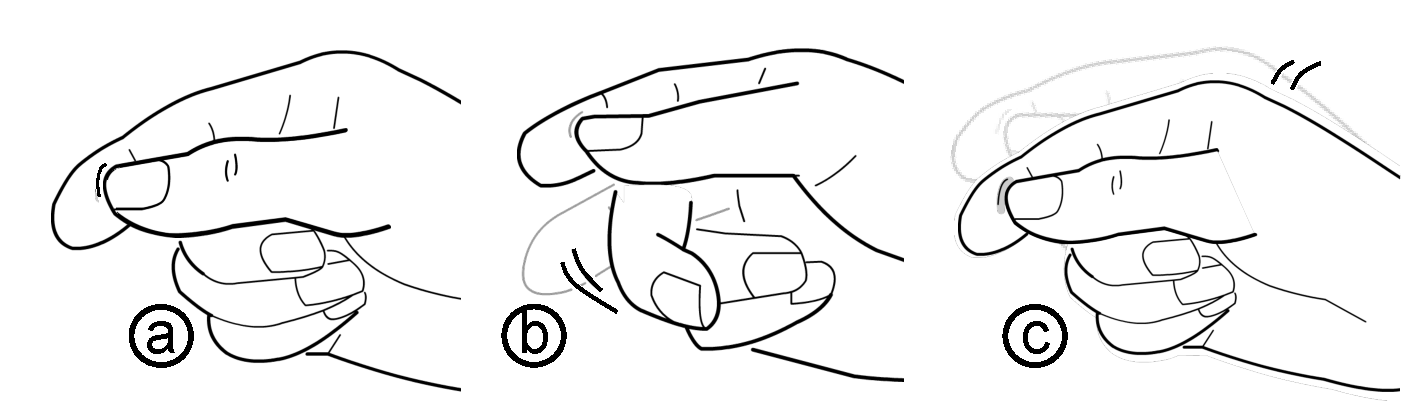
\includegraphics[width=1\linewidth]{clickMethods}\\
   \end{tabular}
\caption{Other commitment methods described by the participants. (a) press (e.g., the mouse button), (b) move the middle finger, and (c) move the wrist.}
\label{fig:clickMethods}
\end{center}
\end{figure}




\section{RELATED WORK}
This work is related to private and subtle interaction, and finger-worn devices, and magnetic tracking.

\subsection{Private and subtle interaction}
%mulscle\cite{Saponas:2009}, nenya\cite{Ashbrook:2011}, iRing\cite{Ogata:2012}, pinstripe\cite{Karrer:2010}
%footSense\cite{Scott:2010}, whack gestures\cite{Hudson:2010}
%pocket touch\cite{Saponas:2011}, ShoeSense\cite{Bailly:2012}, 
Several subtle interaction technique had been proposed. 
Costanza et al.  \cite{Costanza:2007} had used electromyography for sensing subtle motionless gestures. 
Saponas et al. \cite{Saponas:2009} used the similar technique for sensing different finger gestures.  
Scott et al. \cite{Scott:2010} proposed the idea of using mobile devices located in user's pocket to sense the foot gestures.
PingStripe \cite{Karrer:2010} allows users to perfrom subtle interactions by pinching and rolling a piece of their cloths.
Other works \cite{Ashbrook:2011, Ogata:2012} used ring as the subtle input device.
Still, these works can only support limited gesture input. 
FingerPad, on the other hand,  is functionaly equivient to a the touchpad, which implies that providing more dimensions for the input space.

\subsection{Finger-worn input devices}
%fingerRing \cite{Fukumoto:1994}, eyeRing\cite{Nanayakkara:2012}, magicFinger\cite{Yang:2012}, ubiFinger\cite{4030901}, irRing\cite{Roth:2010}
%such as Nenya[N] provide 1D input by rotating the ring on the finger, and iRing [R] additionally allows tapping input through the ring. 
%Disappearing device[D] allows marking menus through one-pixel motion scanner embedded in the ring device.
Several works using the finger-worn devices for sensing gestures had been proposed. 
FingerRing \cite{Fukumoto:1994} placed accelerometers on every finger of user's hand for sensing different chord gestures.     
UbiFinger \cite{4030901} allows users to control house appliances using finger gestures by placing IR transmitter and bending/touch sensors on the index finger in combination with the accelerometer on the wrist.
MagicFinger \cite{Yang:2012} extended the dimensions of touching gestures by mounting camera on the finger.
Since FingerPad using finger pinch gestures as the input, it increases both privacy and subtlety in comparrison to these works. 

%\subsection{Always-available interaction}
%Tracking the high degrees-of-freedom of human hands as inputs, Digits, a wrist-worn mobile hand tracking device, allows users to use full hand gestures on the move. This device, nevertheless, requires high power cameras and suffers from occlusion problem.

%\subsection{Eye-free interaction}

\subsection{Magnetic tracking}
%\neyna, Abracadabra, GaussSense ... 
Maginetic tracking had been used to sense the gestures in a remote distance. 
For instance, Han et al. \cite{4421009} tracked finger-mounted magnet for handwriting input. 
Similarly, Abracadabra \cite{Harrison:2009} used finger-mounted magnet to control the watch device.
Nenya \cite{Ashbrook:2011}, on the other hand, used the magnet mounted in the finger ring to control the device.
Liang et al. \cite{Liang:2012} used magnetic mounted in the stylus and the hull sensor array for enabling input on arbitrary surface.
In comparrison to these works, FingerPad provides more private and subtle input by mounting the hall sensors and magnet on the fingertips.
 

%\subsection{One-handed interaction}
%Others further remove the travel distance by allowing hand gestures. GestureWrist reads gestural input through a capacitive-sensing watch-bend. Digits allows users to use full hand gestures on the move, using a wrist-worn depth sensors. Gesture input, nevertheless, requires to memorize functional mappings. 


%\section{DESIGN}
%Owing to natural bio-mechanism of human hand, use of the index fingertip as a touchpad is not as easy as conventional touch pads. Firstly, unlike flat touch pads, fingertips are soft and curve, causing regions in the fingertip are not equally visible. Secondly, motor space of the two fingers is constrained due to the fact of the index and thumb are mechanically connected by joints. Both make the touch regions in index fingertips not equally attainable.

%To understand how to design touch interface for FingerPad, we conducted a pilot study where we asked participants to rate comfort level in fingertip regions. As illustrated in Figure \ref{fig:pilotStudy}a, the participant, right-handed, was instructed to raise the index finger up front pointing left, suggesting a landscape touchpad, such that they could easily tap with the thumb tip. To guide the participants where to touch in the fingertip, we stick a thin translucent dot patten, in Figure \ref{fig:pilotStudy}b, on their index fingertips. The pattern includes 4 by 4 dots evenly arranged across fingertip as a grid (Figure \ref{fig:pilotStudy}b).

%\begin{figure}
%\begin{center}
%  \begin{tabular}{@{\hspace{0.1cm}}c}
%		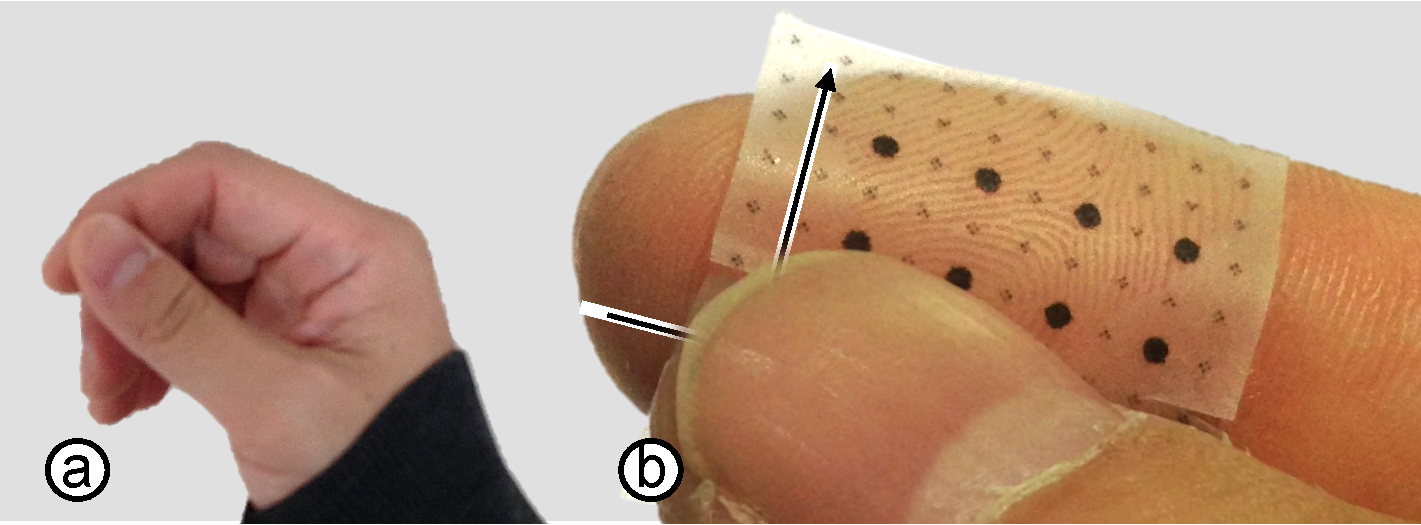
\includegraphics[width=1\linewidth]{pilotStudy}\\
%   \end{tabular}
%\caption{(a) The posture the participants were instructed to perform in the pilot study. (b) The translucent dot pattern stick on the fingertip to guide the participants through touch.}
%\label{fig:pilotStudy}
%\end{center}
%\end{figure}


%\section{DESIGN: IndexPad v.s. ThumbPad}
%Unlike touchpads where the finger is always considered as an input pen, FingerPad's  pad and pen, referring to index and thumb fingertips, are interchangeable. We include two models into consideration: IndexPad and ThumbPad, depending on which fingertip users perceive as the finger touchpad. Misinterpretation of the model applied can lead to inverted results. For example, on a finger pinch, the sense of touch is contributed from the contact regions locating at different parts in the index and thumb fingertips. These regions suggest different touch positions in both fingertips, as well as in the user's mental. Unfortunately, the model applied only exists in users head. Without understanding what might trigger the decision of the model to use, interaction with FingerPad can be frustrating. 

%To understand how users determine which model to use, and what pros and cons each model inherits, we conduct a pilot study.

%We argue that  this decision is affected by the orientations of the fingertips. Unlike touchpads which always face up allowing for touch, the orientation of FingerPad can be various depending on the context of use. The fact that wearing input devices on fingertips suggests using the device instantly at anytime, as shown in Figure \ref{fingerPadPosture}, making this worse.

%Moreover, unlike touchpads which always face up allowing for touch, the orientation of FingerPad can be various depending on the context of use. 
%Depending on the context of use, FingerPad's orientation can be various yet unexpected. 
%The key seems to understand  when and why users perceived their fingertips as the pads.
%Moreover, the fact that wearing input devices on fingertips suggest using it instantly at anytime makes this worse.
%FingerPad allows two distinct interpretations of touch. 

%\label{fig:typeOfPads}

%\subsection{Functional regions}
%Center and upper area receive good comfort level in touch. Lower part is not easily seen. Very lower part often tapping with nail back. Left part taping with thumb tip side. Show several examples in Figure \ref{fig:functionRegion}a.

%As suggesting by the results, we divide the index fingertip into two functional regions: the touch pad , and the bezel buttons, as shown in Figure \ref{fig:functionRegion}b. The pad region suggests a flat surface that maximize visibility and facilitate touch behavior. The bezel regions, on the tip and lower part of the index fingertip, allows buttons to e.g., invoke menus. While the lower part seems wide enough to embed more buttons, we simplify it to single big button because the comfort level is low and the way users might touch it is versatile.

%\begin{figure}
%\begin{center}
%  \begin{tabular}{@{\hspace{0.1cm}}c}
%		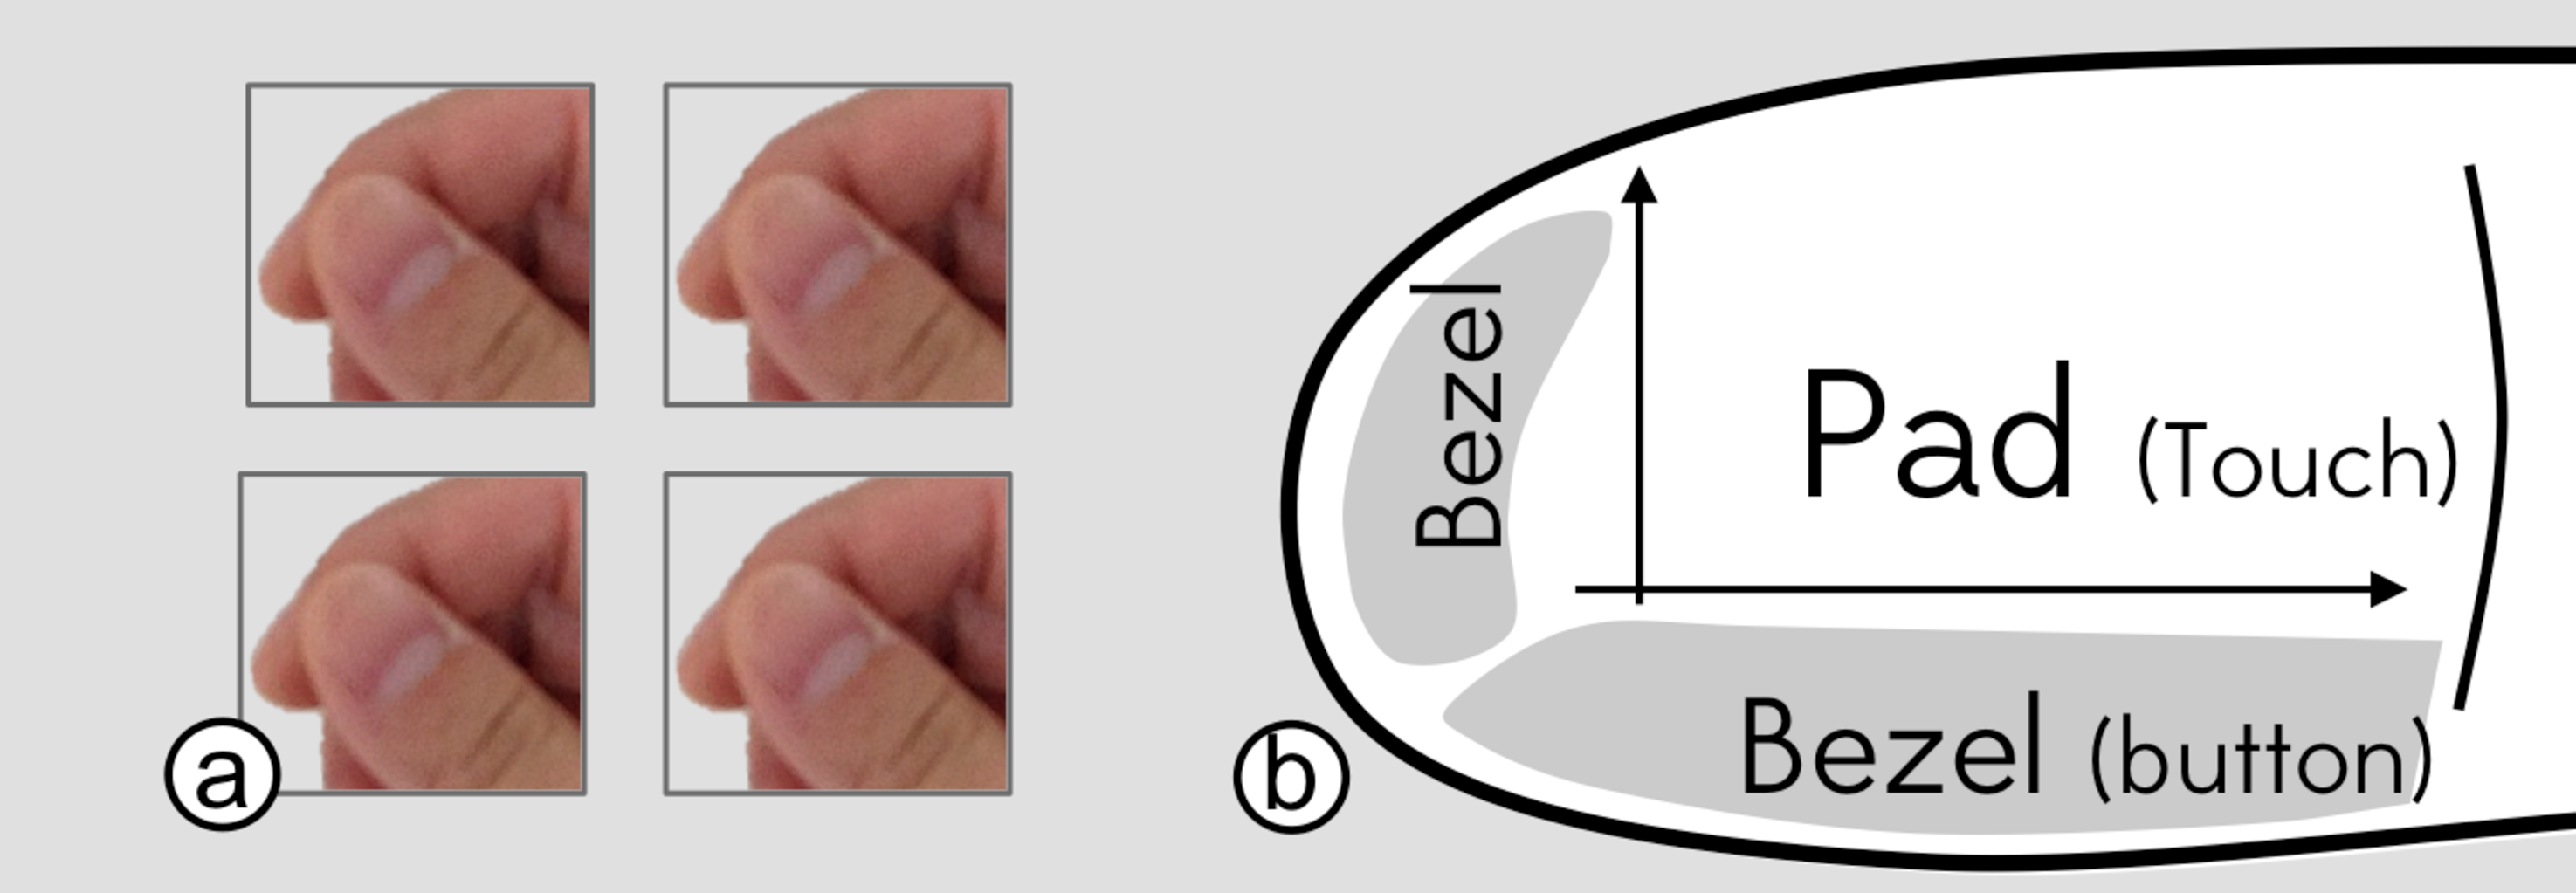
\includegraphics[width=1\linewidth]{fingerpadFunction7}\\
%   \end{tabular}
%\caption{(a) Example postures of the thumb tapping at tip and lower part of the index fingertip. (b)Design of functional regions in FingerPad.}
%\label{fig:functionRegion}
%\end{center}
%\end{figure}


%\section{EXAMPLE APPLICATIONS}
%We present two example applications including one-handed watch, and finger remote.


%\subsection{One-handed watch}
%Current watch displays, such as Sony SmartWatch, use touch screens for user interaction, which force users to operate bimanually (e.g., raise the watch by one hand, and reach to the touch screen by the other). FingerPad allows one-handed touch input using the same hand with watch.
%Two applications are included: photo browsing and instant messaging.
%We map the pad area to touch interface, and the bezel area to side buttons of the watch. 
%The pad area accepts touch positions that are fed to current application, while the bezel area allows for application switch and invoking context menus.

%Conventional applications interfaces that generally require 2D input are provided, including photo browsing, and instant messaging.


%Robin long pressed the index finger pad, followed by a cursor appears on the screen. 

%The user performs (Figure Xa) a slide-to-unlock gesture to activate interactions with the watch. Tapping the side region in bezel area switches from home screen to photo browsing ((Figure Xb). In the pad area, dragging rightward or leftward shows the next or pre photo (Figure Xc), circling to enlarge the current photo (Figure Xd), dragging in enlarge mode to move the viewport,  and double tapping o reset the zooming. To switch albums, the user taps the lower region in bezel area to invoke a menu of albums(Figure Xe) , with which the user further select in the pad area (Figure Xf) .
% Tapping again to the side in bezel are enters instant messaging. Here, dragging to read next message. By invoking the context menu, the user can create, delete, or reply to a  message (Figure Xg) . Uni-stroke input allows the user to enter text information (Figure Xh) .


%\begin{figure}
%\begin{center}
%  \begin{tabular}{@{\hspace{0.1cm}}c}
%		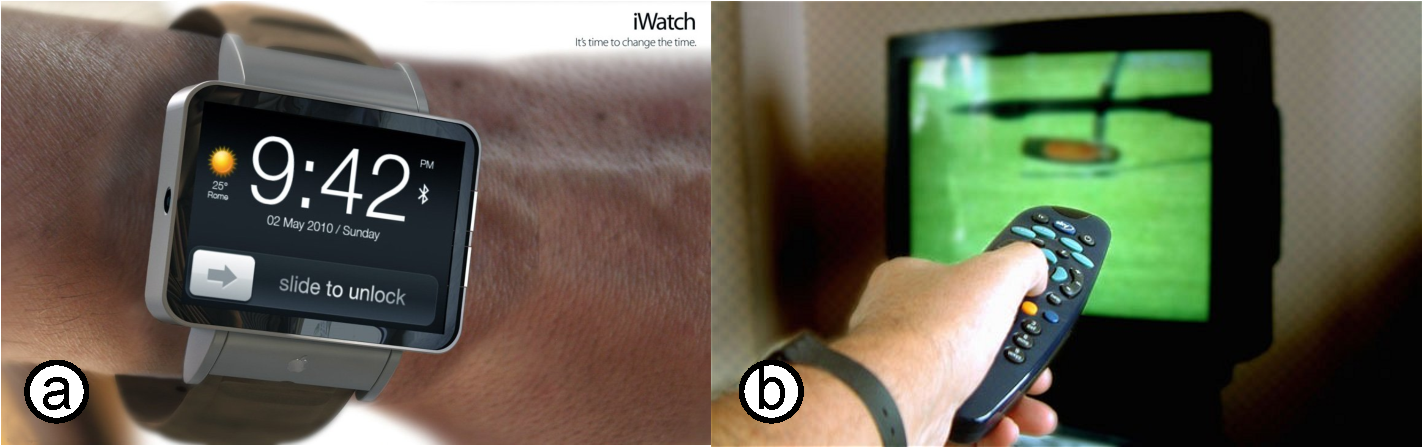
\includegraphics[width=1\linewidth]{applications}\\
%   \end{tabular}
%\caption{Applications of FingerPad.}
%\label{fig:applications}
%\end{center}
%\end{figure}


%\subsection{Finger remote for presentation.}
%FingerPad is instant available, plus the human hand excellent at directional pointing in space, allowing %FingerPad a compelling solution to remote control home appliances in surrounding. We demonstrate %FingerPad as a remote control to home televisions. Basic functions are provided, including volume adjustment and channel switch.

%While the interactions in one-handed watch can be directly used, we add advanced controls in this application. 
%The small fingertip could introduce large CD gain. To avoid xxx, finger remote supports continuing control.
%For example, to jump to a far channel, the user drags on index fingertip to the right and hold for a moment to enter continuing adding. This save the user from multiple crunches. 
%To jump to a certain channel, the user can also write the channel number on the index fingertip.


%\section{ENABLING TOUCH}
%To facilitate the discussion, we describe concerns in prototyping under the context of IndexPad (e.g., regarding index fingertip as touchpad, and thumb tip as the touch pen).

%\subsection{Basic principle}
%The basic idea to determine 
%The basic idea to calculate  position of 
%what are our design requirement? why we choose a not b?

%\subsection{Hardwares in concern}
%\subsubsection{Capacitive sensing}
%\subsubsection{Magnetometer}
%\subsubsection{Hall sensor}


\section{CONCLUSION}
We have presented FingerPad, a nail-mounted device that enables touchpad functions on users index fingertips, allowing for private and subtle interaction on the move. Our studies show user ability in cursor control using the pinch gesture with FingerPad. 
The statistics shows that the users can achieve 93\% accuracy for very small targets (1.2mm) in the seated condition, and 92\% accuracy for 2.5 mm-width target in the walking condition, which is sufficient enough for the mobile usage. 
Through the user study, the design insights are also concluded through the explored three factors, which are the posture, commit method, and target size.
Though there always has the trade-off among the factors, the study still shows that the FingerPad can work very well for the subtle interactions.

For the future, although the design of the FingerPad is for mobile glass display usage, the FingerPad might be also worked without visual supports. 
The different commit methods can also be explored in the future to create more different alternative gestures. 
For the devices designed for richer private output are invented, users have the need to use it privately with richer input device, and moreover, the method should be subtle enough to achieve the social acceptability, such like the FingerPad.   



%We also show how to design a better rich subtle interaction  

 %The result suggested that the FingerPad allows for subtle input through fingertips on the move. 





\section{ACKNOWLEDGMENTS}
This section is left blank for blind review.

%\small
\bibliography{bib}

\end{document}
